% ULaTeX2e, calling the article.cls class and 12-point type.

\documentclass[12pt]{article}

% My packages

\usepackage{framed, color}
\usepackage{soul}
\definecolor{blu}{rgb}{0,0,1}
\newcommand{\td}[1]{{\color{blu}\hl{TODO: #1}}}
\usepackage{graphicx}
\usepackage{amsthm}
\newtheorem{mydef}{Definition}
\usepackage{dcolumn}
\usepackage{multirow}
\usepackage{booktabs}
\newcolumntype{d}{D{.}{.}{4.0}}
\newcolumntype{s}{D{.}{.}{1.4}}

% Users of the {thebibliography} environment or BibTeX should use the
% scicite.sty package, downloadable from *Science* at
% www.sciencemag.org/about/authors/prep/TeX_help/ .
% This package should properly format in-text
% reference calls and reference-list numbers.

\usepackage{scicite}

% Use times if you have the font installed; otherwise, comment out the
% following line.

\usepackage{times}

% The preamble here sets up a lot of new/revised commands and
% environments.  It's annoying, but please do *not* try to strip these
% out into a separate .sty file (which could lead to the loss of some
% information when we convert the file to other formats).  Instead, keep
% them in the preamble of your main LaTeX source file.


% The following parameters seem to provide a reasonable page setup.

\topmargin 0.0cm
\oddsidemargin 0.2cm
\textwidth 16cm 
\textheight 21cm
\footskip 1.0cm


%The next command sets up an environment for the abstract to your paper.

\newenvironment{sciabstract}{%
\begin{quote} \bf}
{\end{quote}}


% If your reference list includes text notes as well as references,
% include the following line; otherwise, comment it out.

\renewcommand\refname{References and Notes}

% The following lines set up an environment for the last note in the
% reference list, which commonly includes acknowledgments of funding,
% help, etc.  It's intended for users of BibTeX or the {thebibliography}
% environment.  Users who are hand-coding their references at the end
% using a list environment such as {enumerate} can simply add another
% item at the end, and it will be numbered automatically.

\newcounter{lastnote}
\newenvironment{scilastnote}{%
\setcounter{lastnote}{\value{enumiv}}%
\addtocounter{lastnote}{+1}%
\begin{list}%
{\arabic{lastnote}.}
{\setlength{\leftmargin}{.22in}}
{\setlength{\labelsep}{.5em}}}
{\end{list}}


% Include your paper's title here

\title{Hysteresis in human computation:\\ how one task affects another} 


% Place the author information here.  Please hand-code the contact
% information and notecalls; do *not* use \footnote commands.  Let the
% author contact information appear immediately below the author names
% as shown.  We would also prefer that you don't change the type-size
% settings shown here.

\author
{Edward Newell, Derek Ruths,\\
\\
\normalsize{\texttt{edward.newell@mail.mcgill.ca}}\\
\normalsize{\texttt{druths@networkdynamics.org}}\\
\normalsize{School of computer science, McGill University,}\\
\normalsize{3630 rue University, Montreal, Quebec, H3A 0C6, Canada}\\
\\
}

% Include the date command, but leave its argument blank.

\date{}



%%%%%%%%%%%%%%%%% END OF PREAMBLE %%%%%%%%%%%%%%%%



\begin{document} 

% Double-space the manuscript.

\baselineskip24pt

% Make the title.

\maketitle 



% Place your abstract within the special {sciabstract} environment.

\begin{sciabstract}

Microtask platforms combine the efforts of large numbers 
of people to perform tasks that are difficult to automate with computers 
alone.  These platforms support near-real-time task completion, mimicking a
compute server, and shift the role of the human from consumer to 
producer of computing resources.  To realize its full
potential, we must understand how human computation differs from machine 
computation, and address the biases inherent in 
human cognition.  The effects of various task-design variables on worker
performance have been investigated, but there has been little 
investigation into how consecutive tasks influence one another. Here we show 
that the responses in later tasks are strongly influenced by the content of 
earlier ones, an effect that is as strong or stronger than the effect of 
framing.  Our findings are not solely cautionary; we find
that these \textit{intertask effects} can be harnessed to improve the quality 
of responses, and might thereby help to achieve expert-level judgments in 
citizen science and other crowdsourcing initiatives. 
As an ancillary contribution, we demonstrate the use of machine learning 
algorithms measure exposure-induced human bias, in terms of its ability to 
influence human computations. 
\end{sciabstract}

\section*{Introduction}
Microtask crowdsourcing platforms like Amazon Mechanical Turk (MTurk) make it 
possible for requesters to submit batches of tasks to a large pool of 
workers, who do the tasks for fun, a sense of purpose, and remuneration 
\cite{kazai2013analysis,Antin20122925}.  
Typical tasks include tagging and categorizing images 
\cite{6116320,Zhai2012357}, transcribing voice recordings 
\cite{chandler2013breaking,paolacci2010running}
or handwritten notes \cite{Berinsky2012351,Finnerty2013}, and judging the 
relevancy of search results 
\cite{le2010ensuring,grady2010crowdsourcing,alonso2009can,kazai2013analysis}.
Originally used to distribute clerical work (\#), these platforms 
increasingly serve as a means to engage experimental participants in a 
research 
setting \cite{paolacci2010running,Berinsky2012351,snow2008cheap,alonso2009can}.
This trend has seeded considerable interest in characterizing the parameters
of task design, and validating the microtask platform methodology (\#).

Computer scientists view microtask platforms in the context of general
computation(\#).  In this regard, the platforms enable a tight integration of 
human and machine computation(\#).  Researchers coined the term HPU 
(Human co-Processing Unit) in analogy to CPUs and GPUs \cite{5543192}.  
Ongoing research pursues the establishment of an HPU instruction set
including basic operators like \texttt{vote}, \texttt{subdivide}, \texttt{map},
\texttt{reduce}, \texttt{sentiment}, and \texttt{image\_tag} (\#).  Libraries 
are being developed to give the programmer more seamless access to HPU 
resources 
 \cite{little2010turkit,minder2011crowdlang,minder2012crowdlang,kittur2011crowdforge}.  
As with other architectures, the HPU architecture makes entirely new classes 
of problems tractable for the programmer (\#).

But the ability to program with high-level human instructions comes with a 
cost: HPU output is inherently noisy (\#).  Part of this noise can be explained
in terms of worker demography (\#).  But systematic cognitive biases also 
play a role (\#).   
So far, investigation has explored how worker performance is influenced by
such design factors as the level of 
pay \cite{kazai2013analysis}, training \cite{le2010ensuring}, pre-screening of 
workers \cite{paolacci2010running}, and user-interface design 
\cite{Finnerty2013}.  Researchers have also investigated \textit{framing}, 
by testing the effects of describing the workflow context 
\cite{Kinnaird2012281}, the purpose of tasks 
\cite{chandler2013breaking}, or using alternate problem descriptions
\cite{thibodeau2013natural}.  To our knowledge, no study has investigated 
the influences that consecutive microtasks exert on one another.

It is known that people are susceptible to priming effects 
\cite{BJOP1796,No2007,beller1971priming}, and, in particular, task-repetition 
effects \cite{Gass1999549,sohn2001task}.  Thus, a worker's response during
one task may depend on previous ones.  Such \textit{intertask} effects
would amount to a kind of \textit{hysteresis}, meaning that HPU outputs are not
only a function of the current input, but also of the history of inputs, with
important implications for the design of crowdsourcing initiatives.

Here we describe a series of experiments, using the Amazon Mechanical
Turk (MTurk) microtask platform (\#), in which we studied intertask effects
for image-labeling tasks.  Image-labeling tasks are among the most 
common kinds of microtasks
\cite{chandler2013breaking,Berinsky2012351,Finnerty2013,paolacci2010running}, 
and it seems likely that this will remain the case in the long term because
they provide a source of ground truth in computer vision research 
\cite{5543192}.  
During the experiments, workers were presented with a series of images (one at
a time), and had to provide five descriptive words (\textit{labels}) for each.
We varied first five images (hereafter the \textit{initial tasks})
and observed the effect this had on the workers' labels for the last five
(\textit{test tasks}).

The initial tasks were chosen to embed a certain \textit{prime concept}.
Our first experiment compares the prime concepts \textit{food} and (non-food) 
\textit{objects}, while our second experiment compares \textit{food} and 
\textit{culture}.  For both experiments, The test tasks used images that
combined both prime concepts used for the initial tasks \td{reword}.  Workers participated 
in only one treatment of one experiment, and were randomly assigned initial 
tasks based on one of the prime concepts.  From the perspective of the worker, 
we made no distinction between the initial tasks and test tasks.

As a point of comparison, we included treatments in which we induced
\textit{framing}. \td{what is framing?}
In the framing treatments, before workers begin the tasks, we told them that 
the purpose of study was to understand the visual perception of 
``food and ingredients'' in one case, or the 
perception of ``objects and tools'' in another.  We varied the language of 
the framing text (hereafter simply the \textit{frame}), and for some treatments
we required the worker to echo the frame using a combo-box input.

We found that intertask effects were stronger than framing, unless the worker
was required to echo the frame, in which case the effects of both exposures were on par.  
Our results demonstrate that initial tasks can change 
workers' focus in later tasks.  Using the wordnet corpus, we analyzed 
the effects on the vocabulary used by workers when 
labeling test tasks. 
Exposure to both framing and initial tasks significantly altered the 
diversity of vocabulary that workers used when referring to the prime concept,
as well as the degree to which workers used specialized (rather than generic) 
words.

Contrary to our initial expectations, our findings suggest that the HPU 
programmer can leverage intertask effects.  By carefully designing workflows,
it is possible to tune worker focus, specificity, and expressivity.  Our 
findings carry two lessons for the task designer: intertask
effects can severely bias HPU output if uncontrolled, but if properly 
controlled, intertask effects might be of significant utility in achieving 
expert-level output.

\paragraph*{Measuring computational hysteresis.}
Before describing the details of our experiments, we explain some 
choices made in measuring intertask and framing effects 
(hereafter collectively \textit{exposure effects}).  
In trying to establish a measure of exposure effects, it might be tempting to 
invoke the notion of a ``neutral frame of mind'' to serve as a baseline. 
But such a concept seems both difficult to define, and unlikely to arise.
Therefore, we always consider the effect of one exposure 
\textit{relative} to another.  We organized our experiments 
into pairs of treatments, between which it is possible to make meaningful 
comparisons.  

Our goal in measuring exposure effects is determine whether they can actually 
alter the course of algorithms.
We could, by means of a $\chi^2$ test, reject the null hypothesis that
differently exposed HPUs have the same distribution of outputs.
However, this alone would not demonstrate a practically significant effect, in 
terms altering the execution path of algorithms.

We developed a more stringent measure in which we train classifier algorithms 
to infer the exposure of an HPU from its outputs.
If a classifier infers an HPU's exposure with significantly 
better accuracy than provided by chance, then the HPU outputs must have 
been affected by the exposure.  
But in addition, the classifier serves as a kind of certificate, since it is 
an example of an algorithm whose path of execution is influenced by the 
exposure of 
individual HPUs.  In the supplementary material, we ground our approach 
rigorously in terms of the L1-distance metric, which is a measure of 
divergence between distributions.  The L1-distance ranges from 
0 to 1.  In our case, a value of 1 indicates that the HPU's exposure
influences its output so strongly that the exposure can be inferred from the
output without ambiguity.  A value of 0 indicates that the exposure has no
impact on the HPU's outputs.  The connection between the
L1-distance, $D_\mathrm{L1}$, and a classifier's accuracy, $\eta$, is given by:
\begin{equation}
	D_\mathrm{L1} \geq 2 \eta - 1, 
	\label{l1}
\end{equation}
Since a classifier's performance provides a lower bound on the L1-distance, 
we shall denote $D_\mathrm{L1}^-\equiv 2\eta-1$.
The L1-distance admits the following interpretation: if two distributions
$P$ and $Q$ have an L1-distance $d$, then in the worst case, the 
frequency with which a binary algorithm operating on samples
from $P$ outputs a 1, will differ from that when operating on samples from 
$Q$ by $d \times 100\%$.  
Thus, we can interpret $D_\mathrm{L1}^-$ as a kind of
lower bound for the worst-case bias induced by HPU hysteresis.
We provide further discussion of the statistical properties of our approach 
in the supplementary material.

\paragraph{Experimental setup.}
\begin{figure}
	\centering
	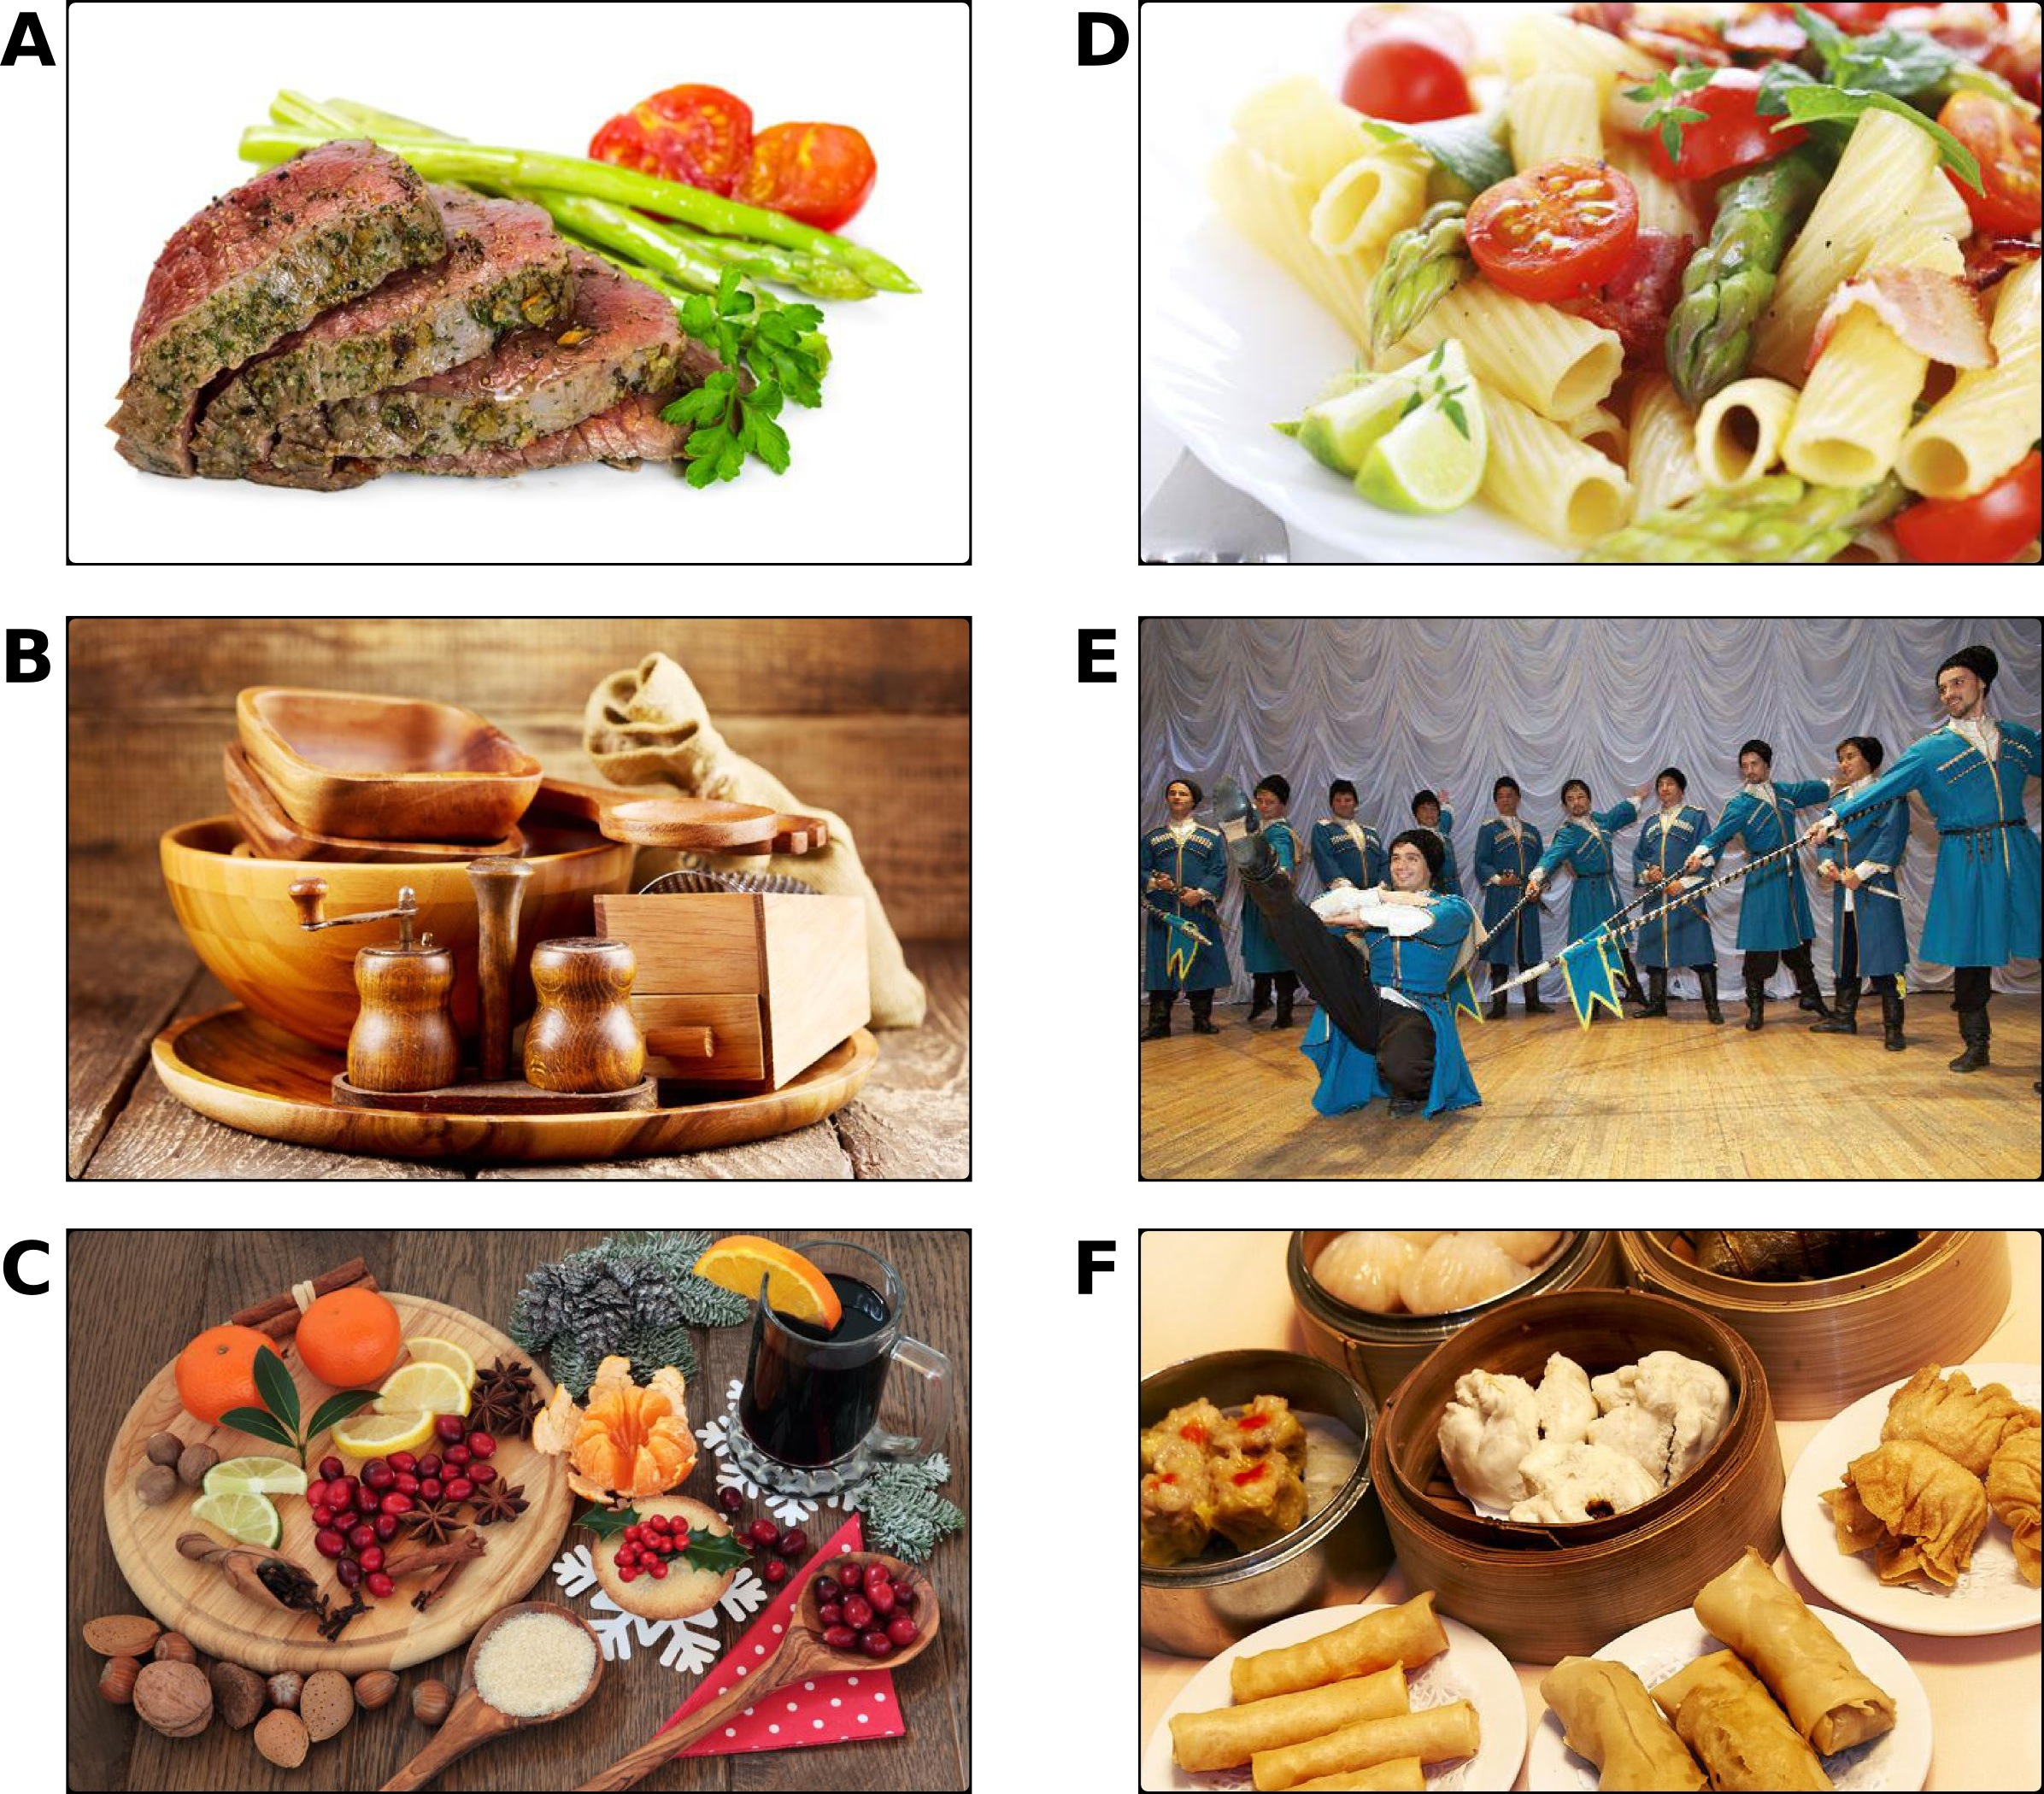
\includegraphics[scale=0.7]{figs/images.pdf}
	\caption{
		Examples of images used in labeling tasks. (The italicized treatment 
		names that follow are defined in Table \ref{table:treatments}.) Images 
		from initial tasks: A) \textit{task1:food}, B) 
		\textit{task1:obj}, D) \textit{task2:food}, 
		E) \textit{task2:cult}.  Images from  test tasks: C) \textit{exp1}, 
		F) \textit{exp2}.  The full set of experimental materials is 
		shown in the supplementary material (S1).
	}

	\label{fig:task}
\end{figure}
We performed two experiments, soliciting respectively 2300, and 900 MTurk 
workers to label images depicting food, kitchen- and dining-ware, and cultural
scenes.  In a given experiment, all workers performed the same test
tasks, the output of which was our main dependent variable.  Before performing
the test tasks, workers were subjected to an exposure, via two 
\textit{modalities}: either they completed a set of initial tasks, or 
were exposed to a frame, or both.  As mentioned, from the perspective of the worker, 
there was no distinction or discontinuity between initial and test tasks.

We organized the experiments into \textit{treatment pairs}.  Both treatments in a 
pair involved the same exposure modality, but differed in the
content of the exposure.  In Table 1, we summarize the various experimental
treatments, and introduce a naming convention that we use to refer to 
treatments and treatment pairs.
In the treatment pairs that studied intertask effects (\textit{task1} and
\textit{task2}), workers performed 10 image-labeling tasks, with the first 
five tasks comprising the initial tasks and the last five tasks comprising the
test tasks.

In the first experiment, the content of the exposures was based on the prime
concepts \textit{food} and \textit{objects} (throughout, ``objects'' should be
taken to imply ``non-edible objects'').  So, 
in \textit{task1:food}, the initial tasks contained images depicting food, 
while in \textit{task1:obj}, they contained images depicting objects, 
including kitchen and dining-ware (see Fig~\ref{fig:task}).  Meanwhile, 
for the exposures in \textit{frame1} we indicating that the study was
``funded by the laboratory for the visual perception of \{ Food and Ingredients
$\vert$ Objects and Tools~\}''.  To further strengthen the frame, we 
introduced another pair of framing treatments, \textit{echo}, with stronger
wording: ``The purpose of this study is to understand the visual perception
of \{ Food and Ingredients $\vert$ Objects and Tools~\}'', and required
the worker to echo the purpose of the study by selecting it among other 
options in a combo-box input.

Note that food and objects are both relatively well-defined classes of 
physical entities.  To explore a different conceptual axis, in 
\textit{exp2} we adopted the prime concepts \textit{food} and \textit{culture}.
Compared to food and objects, culture is more abstract, and, rather than 
comprising a class of physical entities, it encapsulates
sets of beliefs, values, and practices.  Examples of images from the initial 
tasks in \textit{task2} are shown in Fig.~\ref{fig:task}, and the full 
collection of 
experimental materials is presented in the supplementary material (S1).  We 
ensured that all workers only participated in one treatment of one experiment.

\setlength{\tabcolsep}{2pt}
\begin{table}[t]
\centering
\begin{tabular}{ c c c c c }
		\hline \noalign{\smallskip}
		\multicolumn{3}{c}{\textbf{Treatment name}} & \parbox[c]{1.6cm}{\centering \textbf{Frame}} & \parbox[c]{1.3cm}{\centering \textbf{Initial\\ tasks}}	\\ 

		\noalign{\smallskip} \hline \noalign{\smallskip}

		\multirow{6}{*}{ \parbox[c]{0.7cm}{ \phantom{XXX} exp1}} 
			& \multirow{2}{*}{task1} & food & none & food\\
			& & obj & none & objects\\

			\noalign{\smallskip} \cline{2-5} \noalign{\smallskip}
			& \multirow{2}{*}{frame1} & food & food & none\\
			& & obj & objects & none\\

			\noalign{\smallskip} \cline{2-5} \noalign{\smallskip}
			& \multirow{2}{*}{echo} & food & food & none\\
			& & obj & objects & none\\

		\noalign{\smallskip} \hline \noalign{\smallskip}

		\multirow{4}{*}{exp2} 
			& \multirow{2}{*}{task2}  &  food & none & food\\
			& 	&  cult & none & culture\\
			\noalign{\smallskip} \cline{2-5} \noalign{\smallskip}
			& \multirow{2}{*}{frame2} & food & food & food\\
			& 	& cult & culture & food\\

		\noalign{\smallskip} \hline  
	\end{tabular}

	\caption{ \footnotesize{ 
		We use the treatment names shown to refer to specific sections of 
		the data collected.  For example, \textit{task2:food} refers to the
		treatment in the second experiment which was not exposed to a frame, 
		and whose initial tasks contained images of food (7th row).
	}}
	\label{table:treatments}
\end{table}



\paragraph{The strength of intertask effects.}

We assessed the strength of intertask and framing effects
by training a multinomial naive Bayes classifier to infer a worker's exposure
based on the labels provided in the test tasks (see Fig.~\ref{fig:theta}).
This inference was made over the two possibilities for a given treatment pair.
We found that in \textit{task1}, whether a worker performed food- or 
object-containing initial tasks had a strong effect on their subsequent 
labels, introducing a bias that probably exceeds 30\%.  In comparison, the 
framing effect in \textit{frame1} did 
not influence workers' labels enough for the classifier to make predictions 
with significantly better accuracy than that afforded by chance.  The results 
for \textit{exp2} show a similar, but even more pronounced trend, with the bias
induced by intertask effects in \textit{task2} probably exceeding 50\%.

We see a comparable effect size in the \textit{echo} treatment pair.
We expected \textit{echo} to show a very strong effect because, by requiring
the worker to echo the purported purpose of the task, we signal that it
is of particular importance.  The fact that the intertask effects were on par with the framing 
effects in \textit{echo} shows just how powerful intertask effects can be.

\begin{figure}
	\centering
	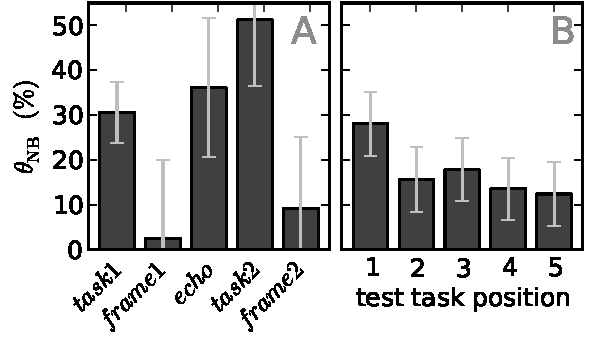
\includegraphics[scale=1]{figs/theta.pdf}
	\caption{
		Lower-bound estimates for the  worst-case bias introduced in image
		labeling tasks due to worker exposure effects.  The estimate was 
		based on the performance of a multinomial naive Bayes classifier,
		trained to infer HPU exposures. A) Bias induced through various
		modalities and prime concepts (see Table 1). B) Bias induced in 
		\textit{task1}, as a function of test task position.  Error bars
		show the one-tailed 95\% confidence interval.
	}
	\label{fig:theta}
\end{figure}

\paragraph{Dynamics of intertask effects.} It is natural to expect 
intertask effects to attenuate as a worker proceeds through the test tasks.  
In \textit{task1}, we permuted the test tasks, allowing us to 
measure intertask effects as a function of task position, while factoring
out the content-dependent differences between tasks
(see Fig.~\ref{fig:theta}B). 
We found intertask effects were most pronounced for the first test task,
dropping off substantially for the second, but maintaining a 
significant effect through until the fifth test task.  
This shows that the range of intertask effects extends across at least five 
tasks, and probably substantially more.
This makes intertask effects of greater concern, but as we will show, it also
makes intertask effects of greater potential utility.
In future work, it would be interesting to investigate whether a worker's
susceptibility to intertask effects varies across a large batch.  For example,
It is conceivable that the first few tasks induce especially strong
or long-lasting effects, in effect ``setting the tone'' for the rest of the batch.

\paragraph{Detailed influences on worker outputs.} 
\begin{figure}
	\centering
	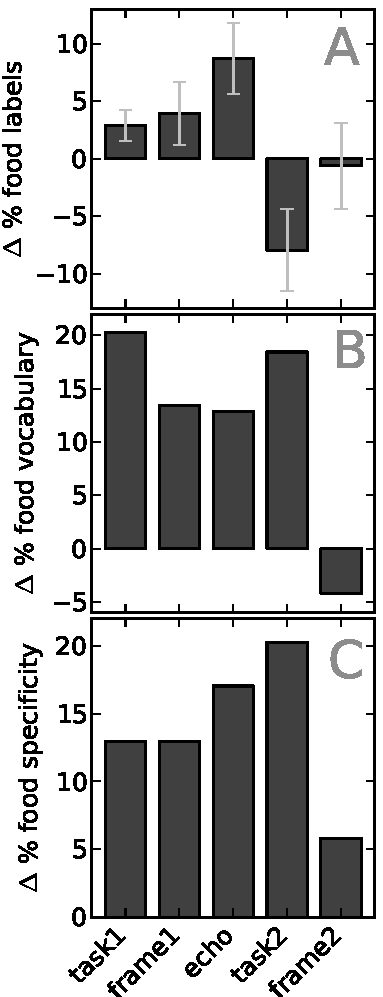
\includegraphics[scale=1]{figs/vocab_specificity.pdf}
	\caption{
		Detailed exposure effects on workers' label vocabulary, for various
		exposure modalities and prime concepts (see Table 1).  A) Change in 
		the number of food-related labels used. B) Change in the total number 
		of \textit{unique} food-related labels used. C) Relative specificity
		of treatment pairs, when considering food-related labels.  For all
		plots, a positive bar height indicates an increase for the 
		food-exposed treatment for the pair indicated on the abscissa.
	}
	\label{fig:specificity}
\end{figure}

Having observed significant effects from framing and task-exposure,
we looked in greater detail at the nature of the effects.  For instance,
does a food-oriented exposure induce workers to provide more food-related
labels?  And if so, does this explain the classifier's ability to distinguish
a worker's initial exposure? 

To answer these questions, we used the wordnet corpus, augmented with names of
ethnic foods learned from the Internet.  Wordnet provides a (roughly)
hierarchical set of relationships between nouns, called hypernym-hyponym
relationships.  A hypernym is a generalization, while a hyponym is a 
specialization.  So, for example, ``bread'' is hypernym to ``rye bread'' 
and hyponym to ``baked goods''.

Using the augmented hypernym-hyponym structure of wordnet to identify nouns 
depicting food, we found that, for the experimental pairings in 
\textit{exp1}, the
food-exposed treatments did produce a significantly larger fraction of 
food-related labels (see Fig.~\ref{fig:specificity}A).  While the shift in 
focus with regard to food does help explain the classifier's ability to 
infer worker exposures, it is insufficient to explain the observed performance
(*).
Furthermore, in \textit{exp2:task2} we see a significant but reversed effect
(see Fig.~\ref{fig:specificity}A), which suggests a more complicated 
relationship between exposure and label usage.
Given the difference between the food-culture and food-object conceptual axes, 
it should perhaps not be surprising that the effect of initial task exposure 
is different.  It would appear that we must be prepared to accommodate 
multiple 
countervailing factors influencing the number of references to the prime 
concept (food).  We will come back to this point momentarily.

To explore these effects further, we looked more closely at which particular
labels were most suppressed (activated) by a worker's exposure.  Remarkably,
we found that, for all treatment pairs, ``food'' was always the most 
suppressed label among 
the food-exposed workers.  This is surprising, considering 
that the overall incidence of food-related labels mostly \textit{increased} 
among food-exposed workers.  But taken together, the increase in references to 
food 
and the decrease in the incidence of ``food'' per se (which is the most generic
food-reference in the wordnet-based ontology), necessarily implies that
food-exposed workers have opted for more specialized references in place of 
``food''. 

In a crowdsourcing task, considerable effort must be given to shaping the 
vocabulary with which a worker engages a task.  To draw an example from the 
domain of citizen science, in galaxy zoo, workers catalog images of galaxies 
in terms of \textit{smoothness}, and the presence of \textit{rings}, 
\textit{dust lanes}, \textit{digital disturbances}, and so on.  Shaping this 
vocabulary is crucial to the reliability of results.  The interface of
galaxy zoo helps by constraining and prompting the user with this basic 
vocabulary.  But this would not appear to be sufficient, since
a set of positive and negative training examples are used, together with
peer-to-peer and peer-to-expert exchange in discussion areas, presumably to
further refine and standardize the vocabulary (\#).  

In our set-up, where the worker's vocabulary is unconstrained, we can 
directly observe the effects that frames and initial tasks have on worker 
vocabulary.  By looking at the number of unique food-related labels that 
workers produced, we assessed the richness of vocabulary that workers used when
referring to food (see Fig.~\ref{fig:specificity}B).  We found that the 
food-exposed workers use a richer vocabulary of 
food-related words, even in cases like \textit{task2:food}, where they 
made fewer references to food overall.  
Interestingly, task-based exposure to food had a stronger enriching effect 
 than did framing-based exposures. (* explain why vocab 
diversity is useful.) 

Using the ontology of food induced by wordnet, along with foods learned from
the Internet, we were able to directly calculate the relative specificity of 
workers from different treatments.
To do this, we considered all the labels from one treatment
(for example \textit{task1:food}) and compared these to all the labels from 
another (\textit{task1:obj}).  For all possible comparisons, we observed 
which treatment's label was more specific more often, and normalized this
quantity as a percentage (we provide greater detail in the supplementary 
material).

We calculated the relative specificity for all treatment pairs, while 
restricting focus to 
food-related labels (see Fig.~\ref{fig:specificity}C).  We found that 
the food-exposed workers always provided food-references of substantially 
greater specificity.  Workers that had labeled images containing food 
were about 12\% more specific than those that labeled images of objects,
and about 20\% more specific than those that labeled images of cultural 
scenes.  With respect to the specificity of food references, framing effects 
were on par with intertask effects.

Taken together, the results presented in Fig.~\ref{fig:specificity} can 
be explained by a combination of priming and  \textit{negative} priming.
Negative priming occurs when a repeated stimulus, which is perceived to be
non-salient, begins to be ignored (\#).  

We propose that, as a worker from \textit{task1:food} proceeds through the 
initial tasks, food-related memories and concepts are activated, increasing 
the likelihood that she uses a variety of food-related labels.  This accounts
for the overall increases the number of food-related labels, as well as the 
richness and specificity of her food-related vocabulary.  At the same time,
since all images up to that point contained food, \textit{whether or not}
an image contains food begins to appear non-salient, suppressing the most 
generic references, such as ``food''.  Thus, there is a simultaneous emphasis of the specialized 
references to the prime concept and de-emphasis of generic references. 

This view can account for the observation that there are fewer
food-related references overall in \textit{task2:food} compared to 
\textit{task2:cult}.  Workers in \textit{task2:food}, like those in 
\textit{task1:food}, are primed to use
specialized food references and negatively primed against using generic
ones.  Then, when these workers encounter the test tasks, with images 
containing more prominent cultural content, they attend to this novel content, 
decreasing their balance of food references.  
Meanwhile, workers in \textit{task2:cult}, having seen only cultural scenes,
experience novelty from the appearance of food-oriented content in the test 
tasks, and, attending to it, drive the relative difference in the quantity of 
food-related labels further toward the negative in in 
Fig.~\ref{fig:specificity}A.

Based on these observations, we submit the following ideas for consideration 
by the designers of crowdsourced initiatives.
\begin{enumerate}
	\item{
		Training tasks should be preferred over examples, since the immediate
		active use of information appears to increase its impact.
	}
	\item{
		Training tasks should contain the same distribution of 
		noise (or ``distracting features''), as the real dataset.
		Exposing workers to irrelevant features, and identifying them as such,
		will free up worker attention for salient features, by virtue of
		negative priming.
	}
	\item{
		\textit{Validation tasks}, for which the correct output is known,
		are often used as a quality control measure.
		These should be dually considered as \textit{calibration tasks}, and
		should be designed to help workers maintain an optimally primed 
		state. Feedback, for both correct and incorrect responses, 
		may further reinforce salient features.
	}
	\item{
		In many applications, such as the detection of pre-ictal 
		(pre-seizure) EEG traces, workers encounter few positive examples
		(most traces are not pre-ictal)(\#).  In the absence of positive 
		examples, the target concept may degrade or drift.
		Drawing calibration tasks from the underrepresented class may 
		help sustain the target concept.
	}
	\item{
		For the most precise classifications, it may be helpful to
		begin with a coarse classification.  For example, workers could 
		initially choose from  \texttt{class0}, \texttt{class1}, and 
		\texttt{borderline}.  Following the coarse classification, the 
		\texttt{borderline} examples could be batched together, allowing 
		workers to focus on features that are only salient for such fine 
		distinctions.
	}
\end{enumerate}

These recommendations follow logically from our observations, but they are 
educated guesses.  We leave their direct testing to future work.

\paragraph{Conclusion.}
Our results show that intertask effects are 
as strong as framing effects, and are stronger when the frame is not echoed.
Our analysis using wordnet reveals that intertask and framing effects
act on workers' vocabulary in subtle ways.  Both exposure modalities 
increased the richness of workers' vocabulary in reference to the prime 
concept, but more so in the case of task-based exposure.  Both modalities 
also increased the specialization of workers' vocabulary in reference to the 
prime concept.

We recommend that intertask effects be considered when designing crowdsourced
studies.  Despite efforts to eliminate biases from the context of tasks,
the greatest source of biases may lurk in the tasks themselves.
At the same time, their positive effects on workers' vocabulary suggest 
that, when properly controlled, intertask effects may be
used to optimize HPU performance.  Based on the enriching effects we observed
for worker vocabulary, intertask effects might be leveraged to achieve 
expert-level annotation in a wider variety of applications.

\bibliography{newbib}
\bibliographystyle{Science}


\section*{Supplementary Material}

\subsection*{S1: Experimental materials}
The tasks for both experiments were presented as a series of slides.  In
both cases, the first slide consisted of a brief set of instructions, followed
by the frame if shown (only some treatments involved a frame), see 
Fig. S\ref{fig:hit_preamble}.  Following the instructions and prime, a set
of initial tasks was shown (except for the treatments in \textit{frame2}
and \textit{echo}) followed by (in all cases) a set of test tasks.  In
\textit{exp1}, two kinds of frame were used, one simple frame, and one where
the worker was required to echo the frame using a combo-box input.  The
instructions, both kinds of frame, and an example task slide, are shown 
in Fig. S1.
\begin{figure}
	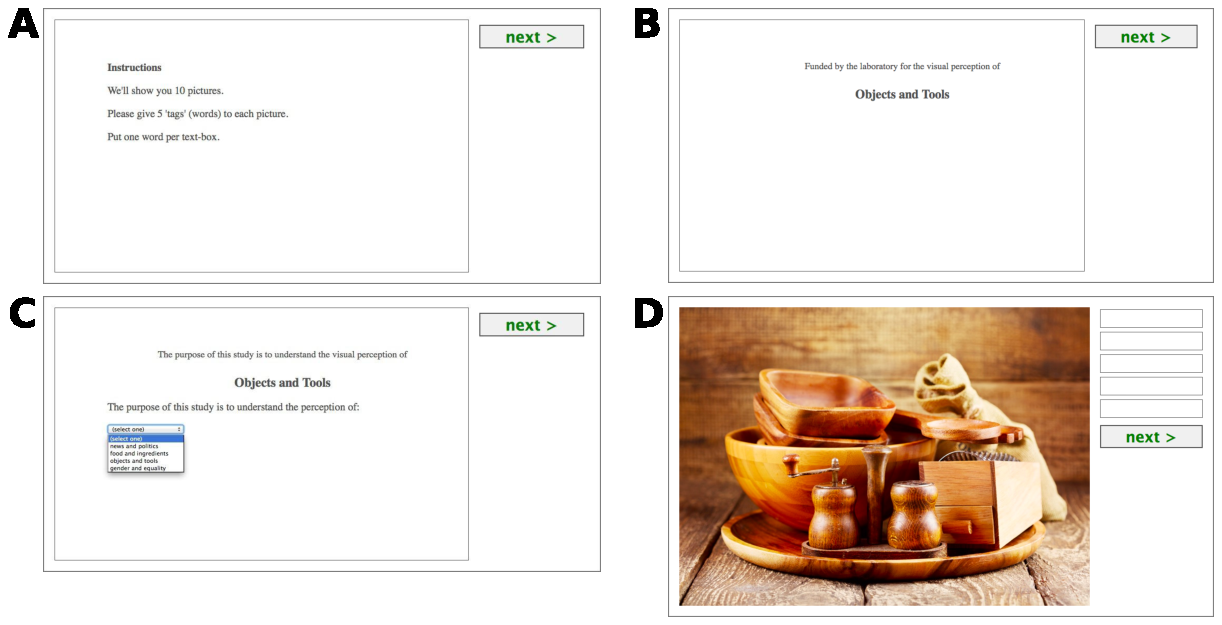
\includegraphics[scale=0.8]{figs/tasks.pdf}
	\label{fig:hit_preamble}
	\caption{Examples of A) instructions; B) a frame, as shown in 
		\textit{frame1:obj}, and similar to those shown in 
		\textit{frame1:food} and \textit{frame2:food}, and 
		\textit{frame2:cult};  
		C) an echoed frame, as used in \textit{echo:obj}, and similar to that
		used in \textit{echo:food}; and D) an 
		example of an image labeling task.
	}
\end{figure}

All of the initial tasks had the format shown in Fig. S1D.  The images used
in the initial tasks for \textit{task1:food} and \textit{task1:obj} are
shown in Fig. S2 and S3, and the images used in the test tasks for 
\textit{exp1} are shown in Fig. S4.  The images used in the initial tasks
for \textit{task2:food} and \textit{task2:cult} are shown in Fig. S5 and
Fig. S6 respectively, and the images used in the test tasks for \textit{exp2} 
are shown in Fig. S7.

\begin{figure}
	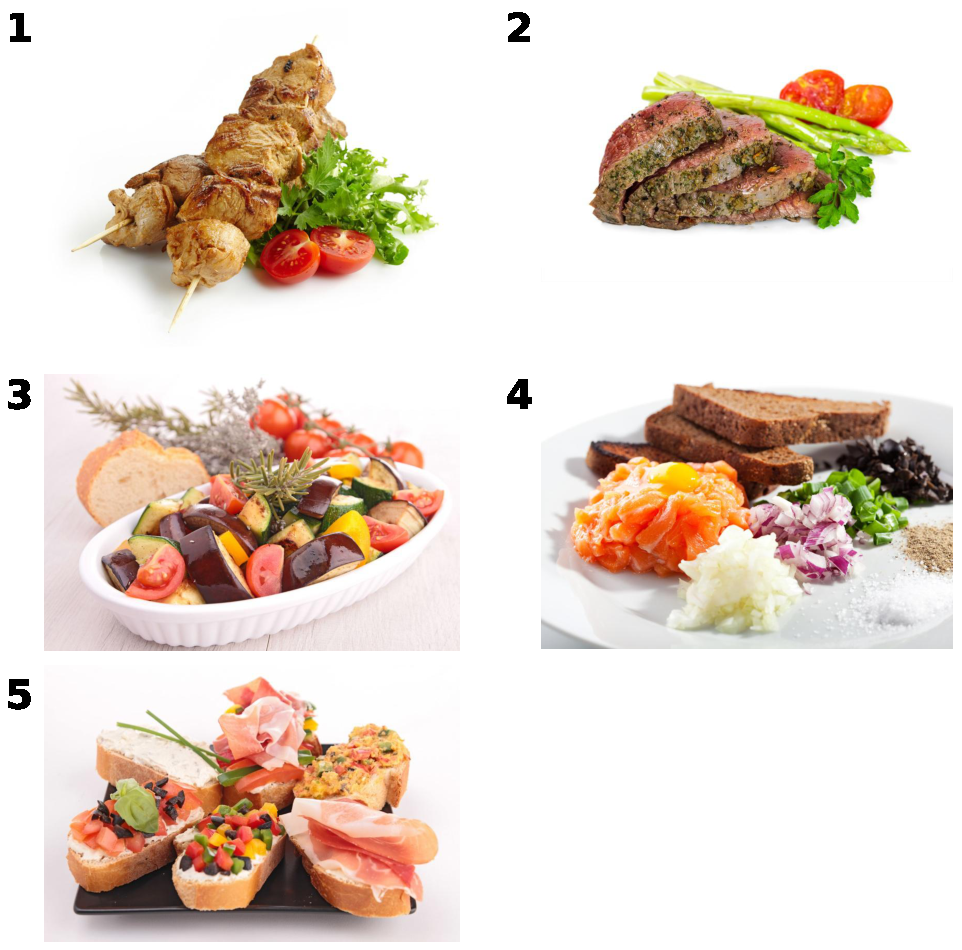
\includegraphics{figs/task1-food.pdf}
	\label{fig:task1:food}
	\caption{
		Figure S2: Images used in the initial tasks for 
		\textit{task1:food}.  The numbers show the order in which the 
		images were presented to workers.
	}
\end{figure}

\begin{figure}
	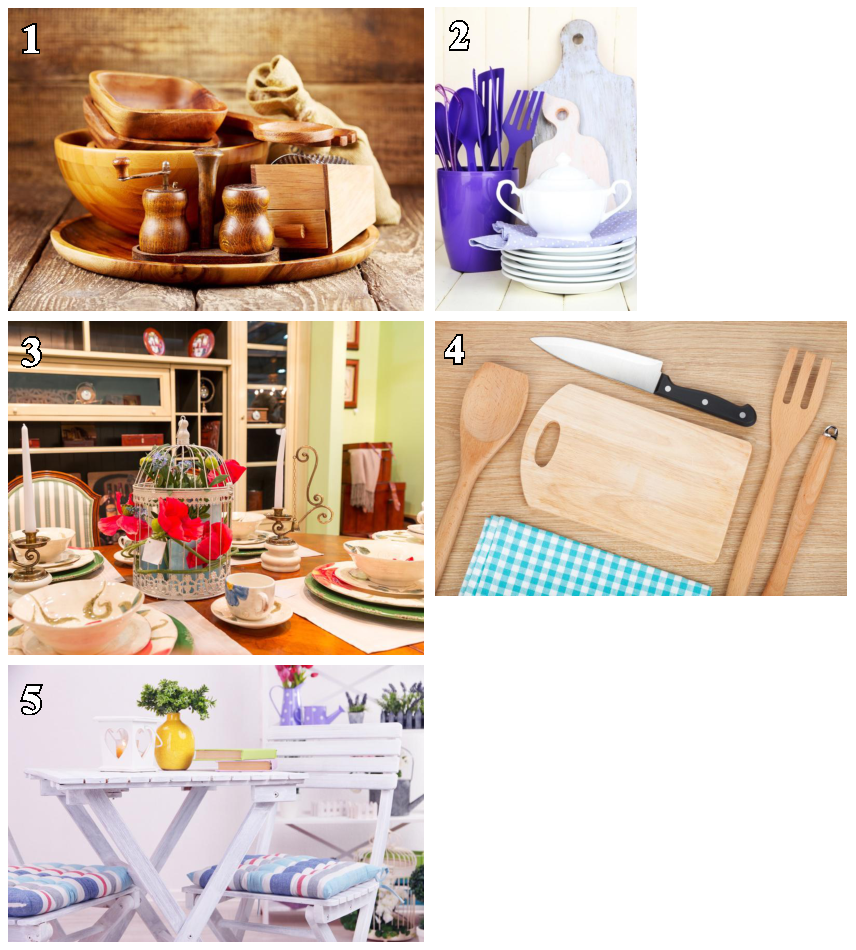
\includegraphics{figs/task1-obj.pdf}
	\label{fig:task1:obj}
	\caption{
		Figure S3: Images used in the initial tasks for 
		\textit{task1:obj}.  The numbers show the order in which the 
		images were presented to workers.
	}
\end{figure}

\begin{figure}
	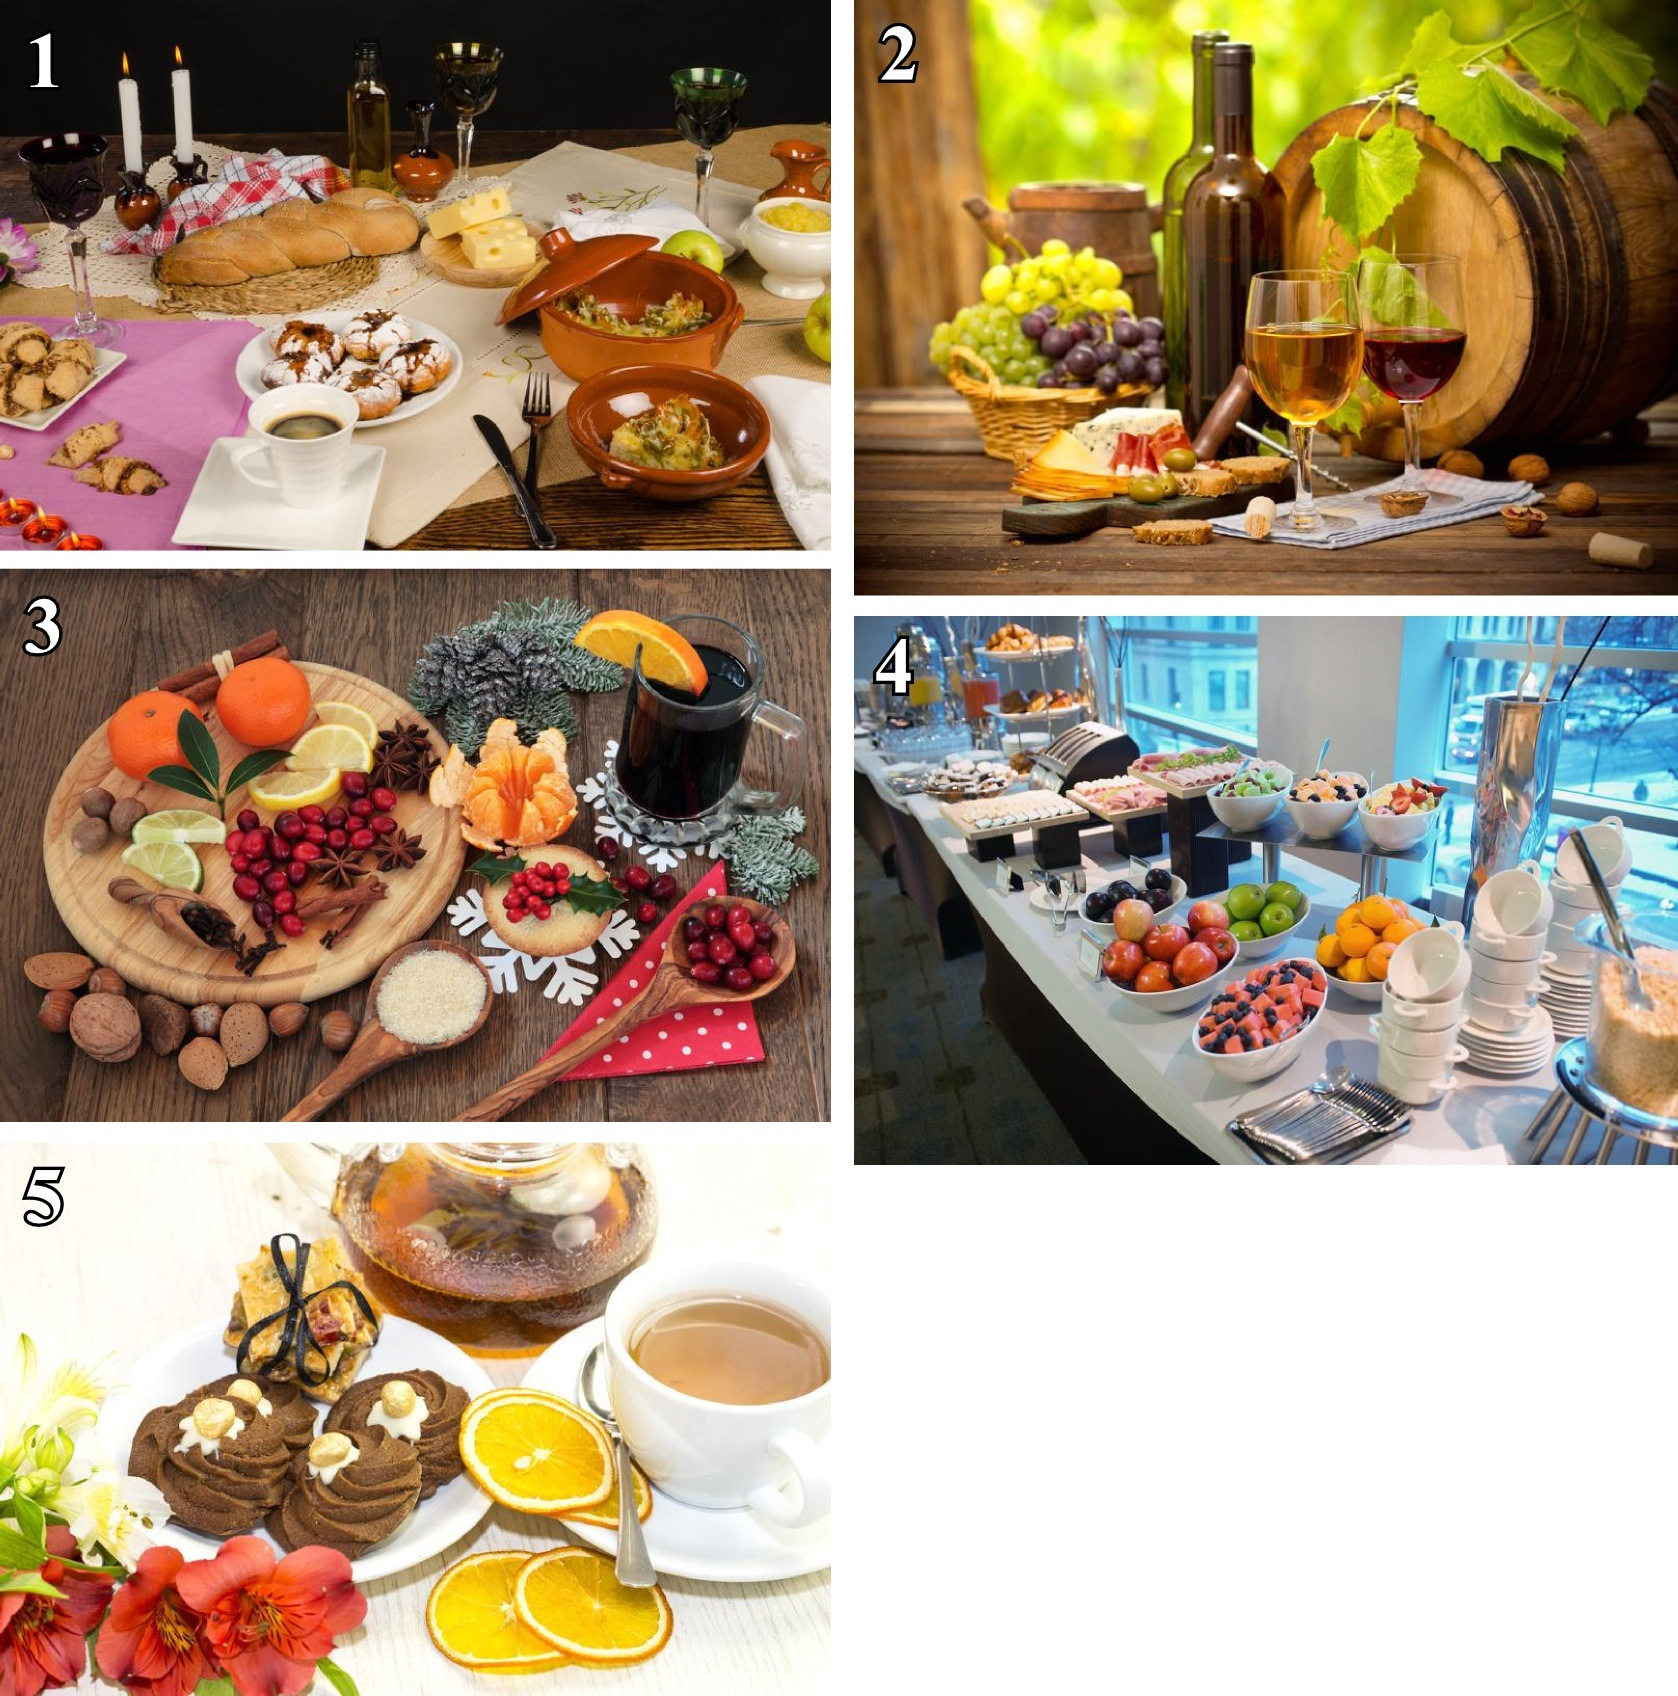
\includegraphics{figs/task1-test.pdf}
	\label{fig:task1:test}
	\caption{
		Figure S2: Images used in the test tasks for 
		\textit{exp1}.  The numbers show the order in which the 
		images were presented to workers.
	}
\end{figure}

\begin{figure}
	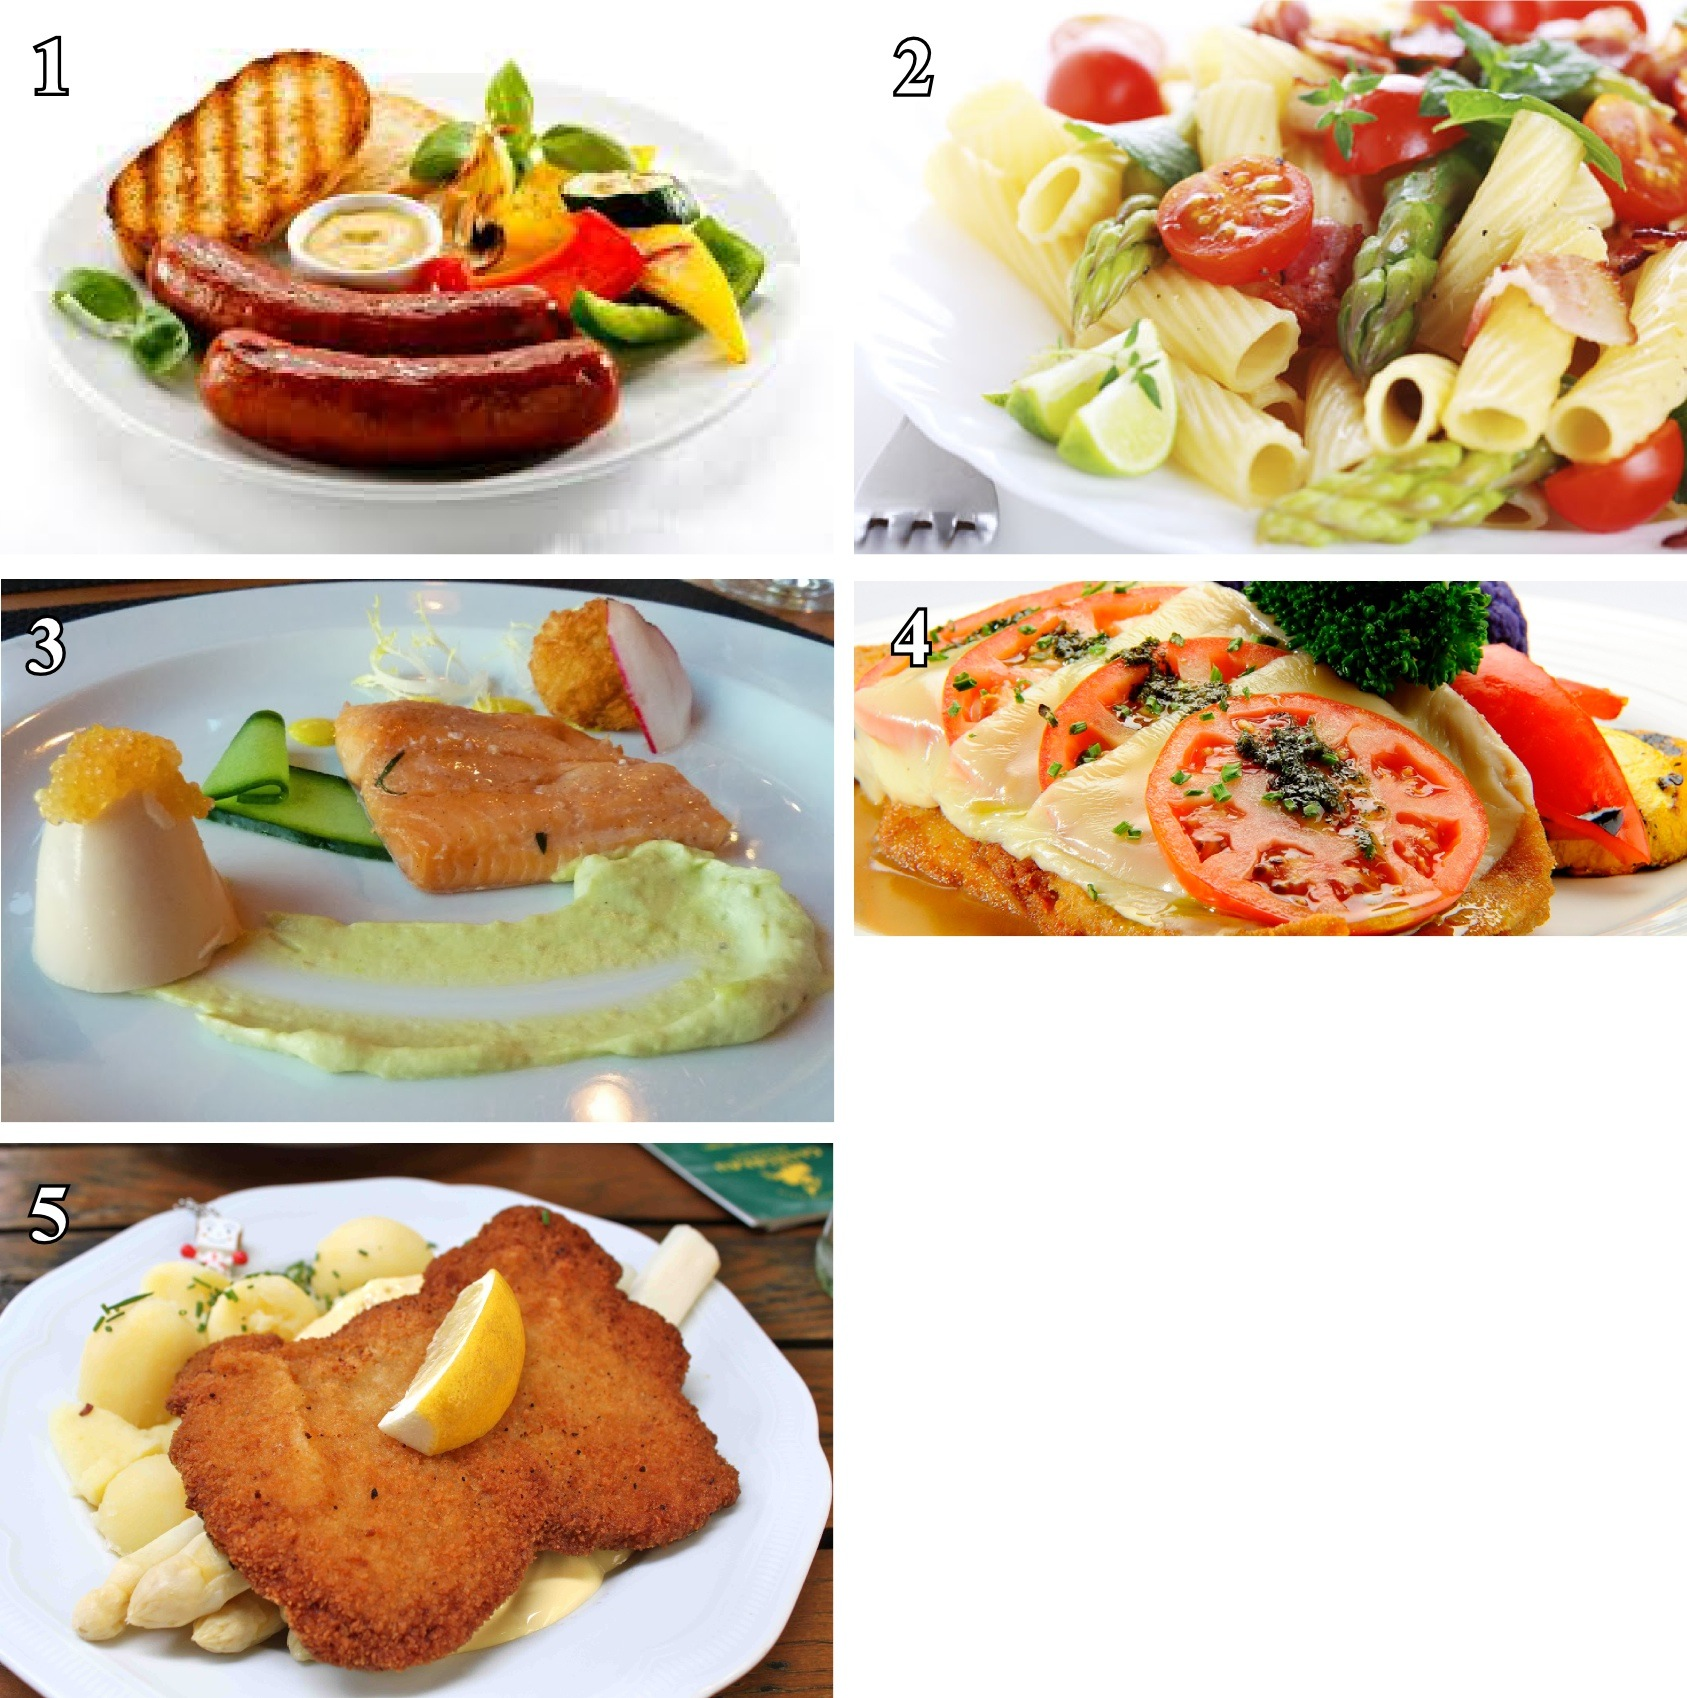
\includegraphics{figs/task2-food.pdf}
	\label{fig:task2:food}
	\caption{
		Figure S2: Images used in the initial tasks for 
		\textit{task2:food}.  The numbers show the order in which the 
		images were presented to workers.
	}
\end{figure}

\begin{figure}
	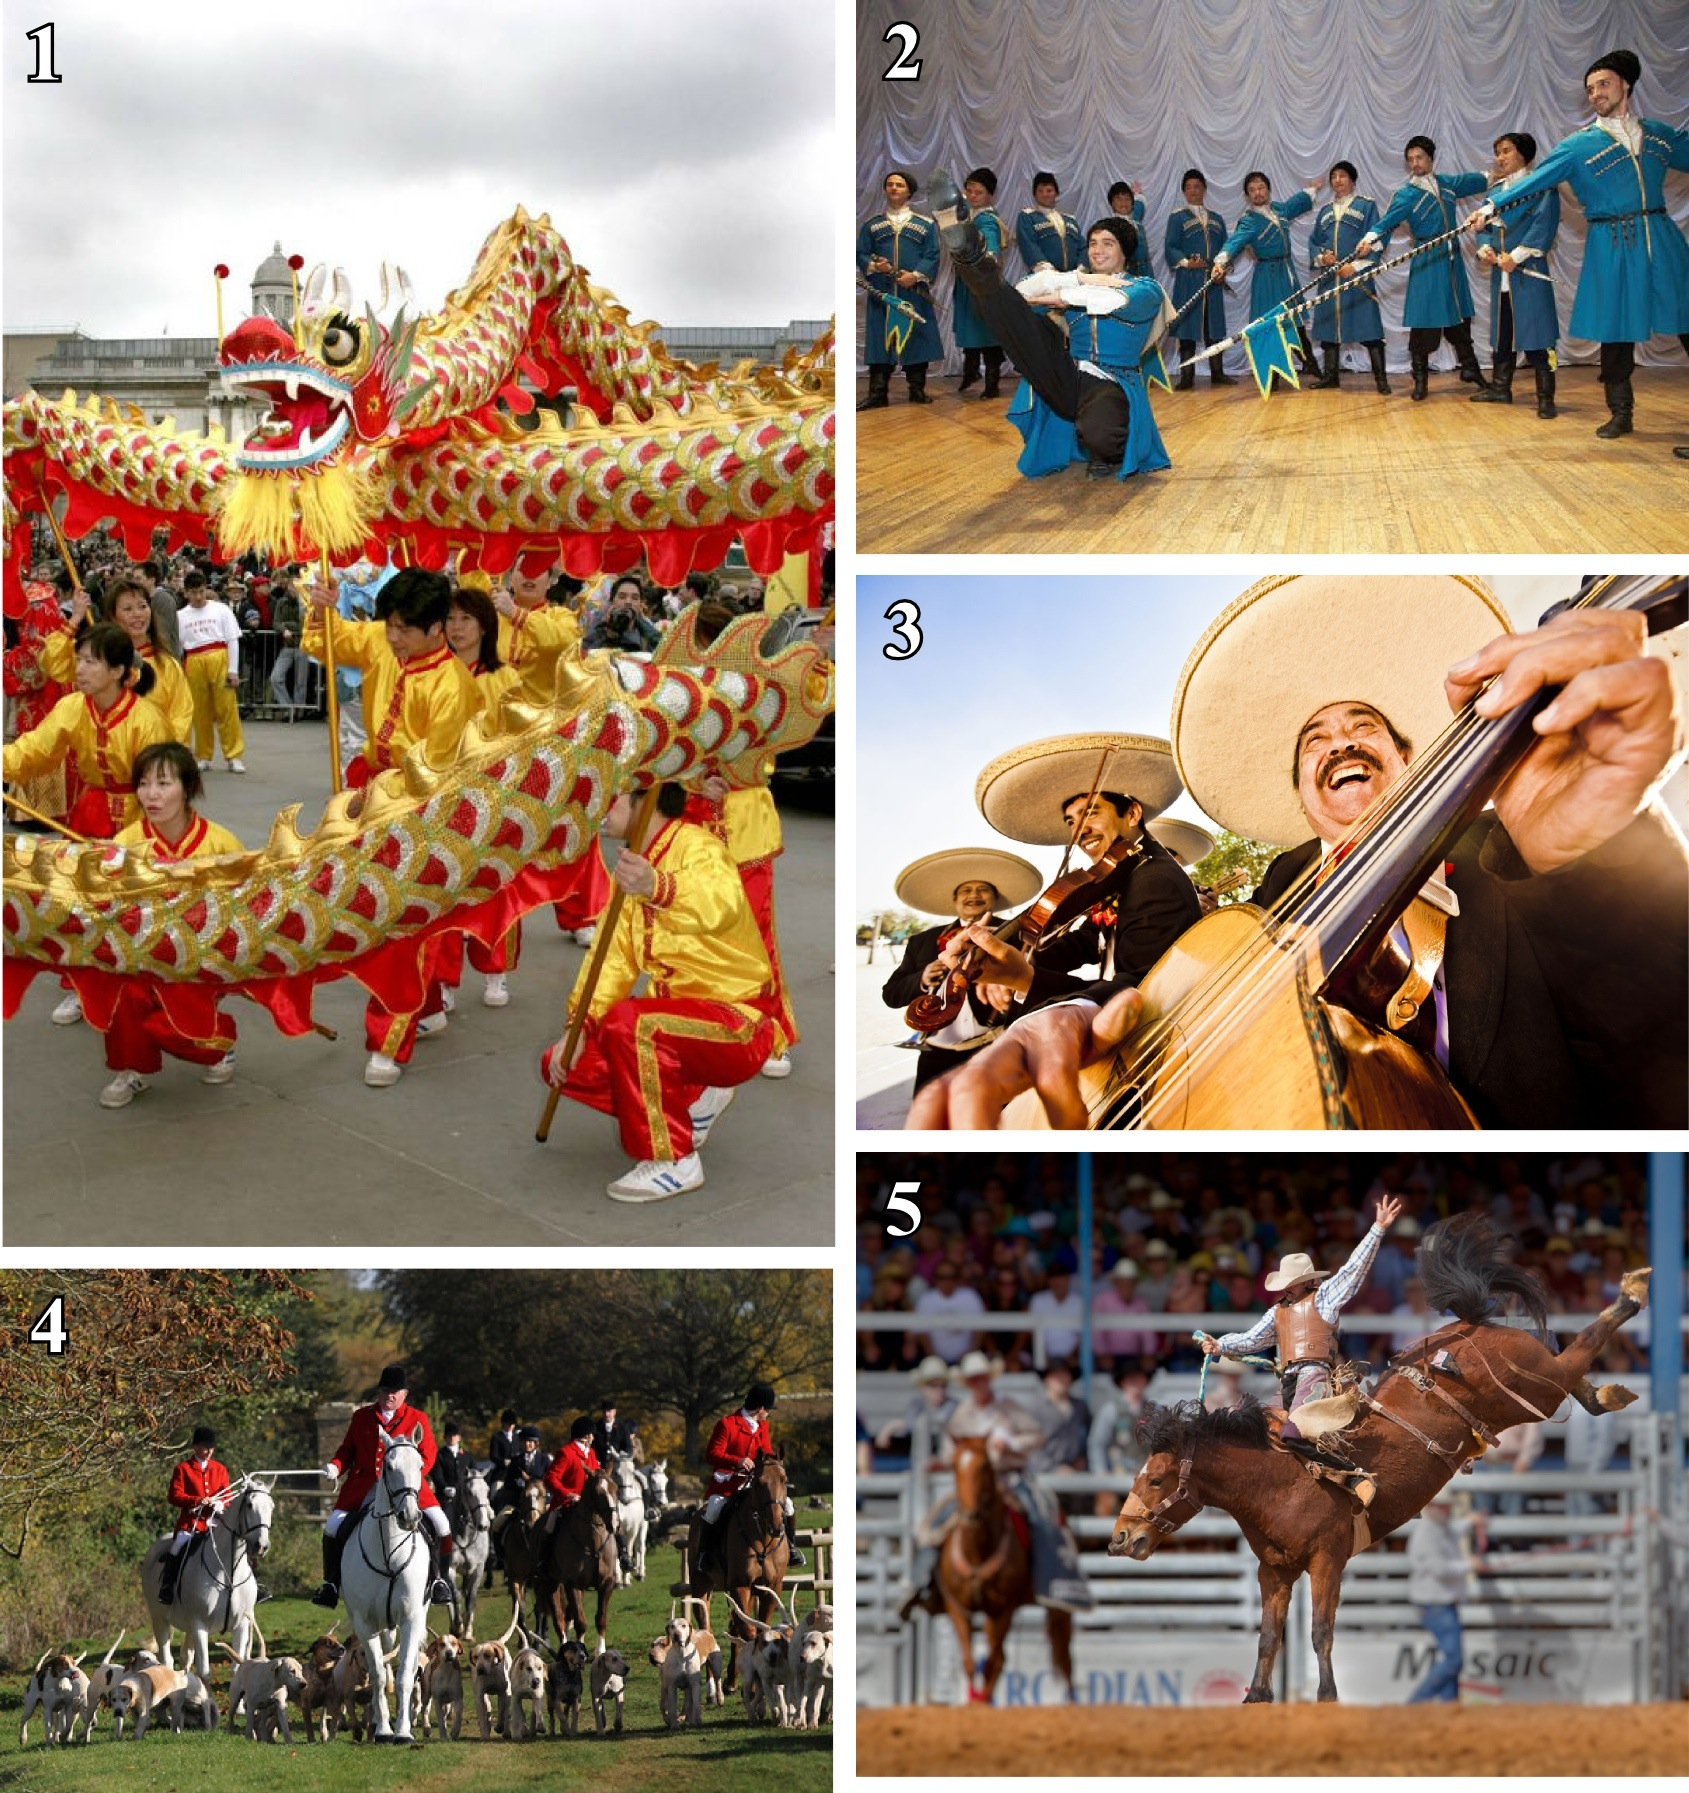
\includegraphics{figs/task2-cult.pdf}
	\label{fig:task2:cult}
	\caption{
		Figure S2: Images used in the initial tasks for 
		\textit{task2:cult}.  The numbers show the order in which the 
		images were presented to workers.
	}
\end{figure}

\begin{figure}
	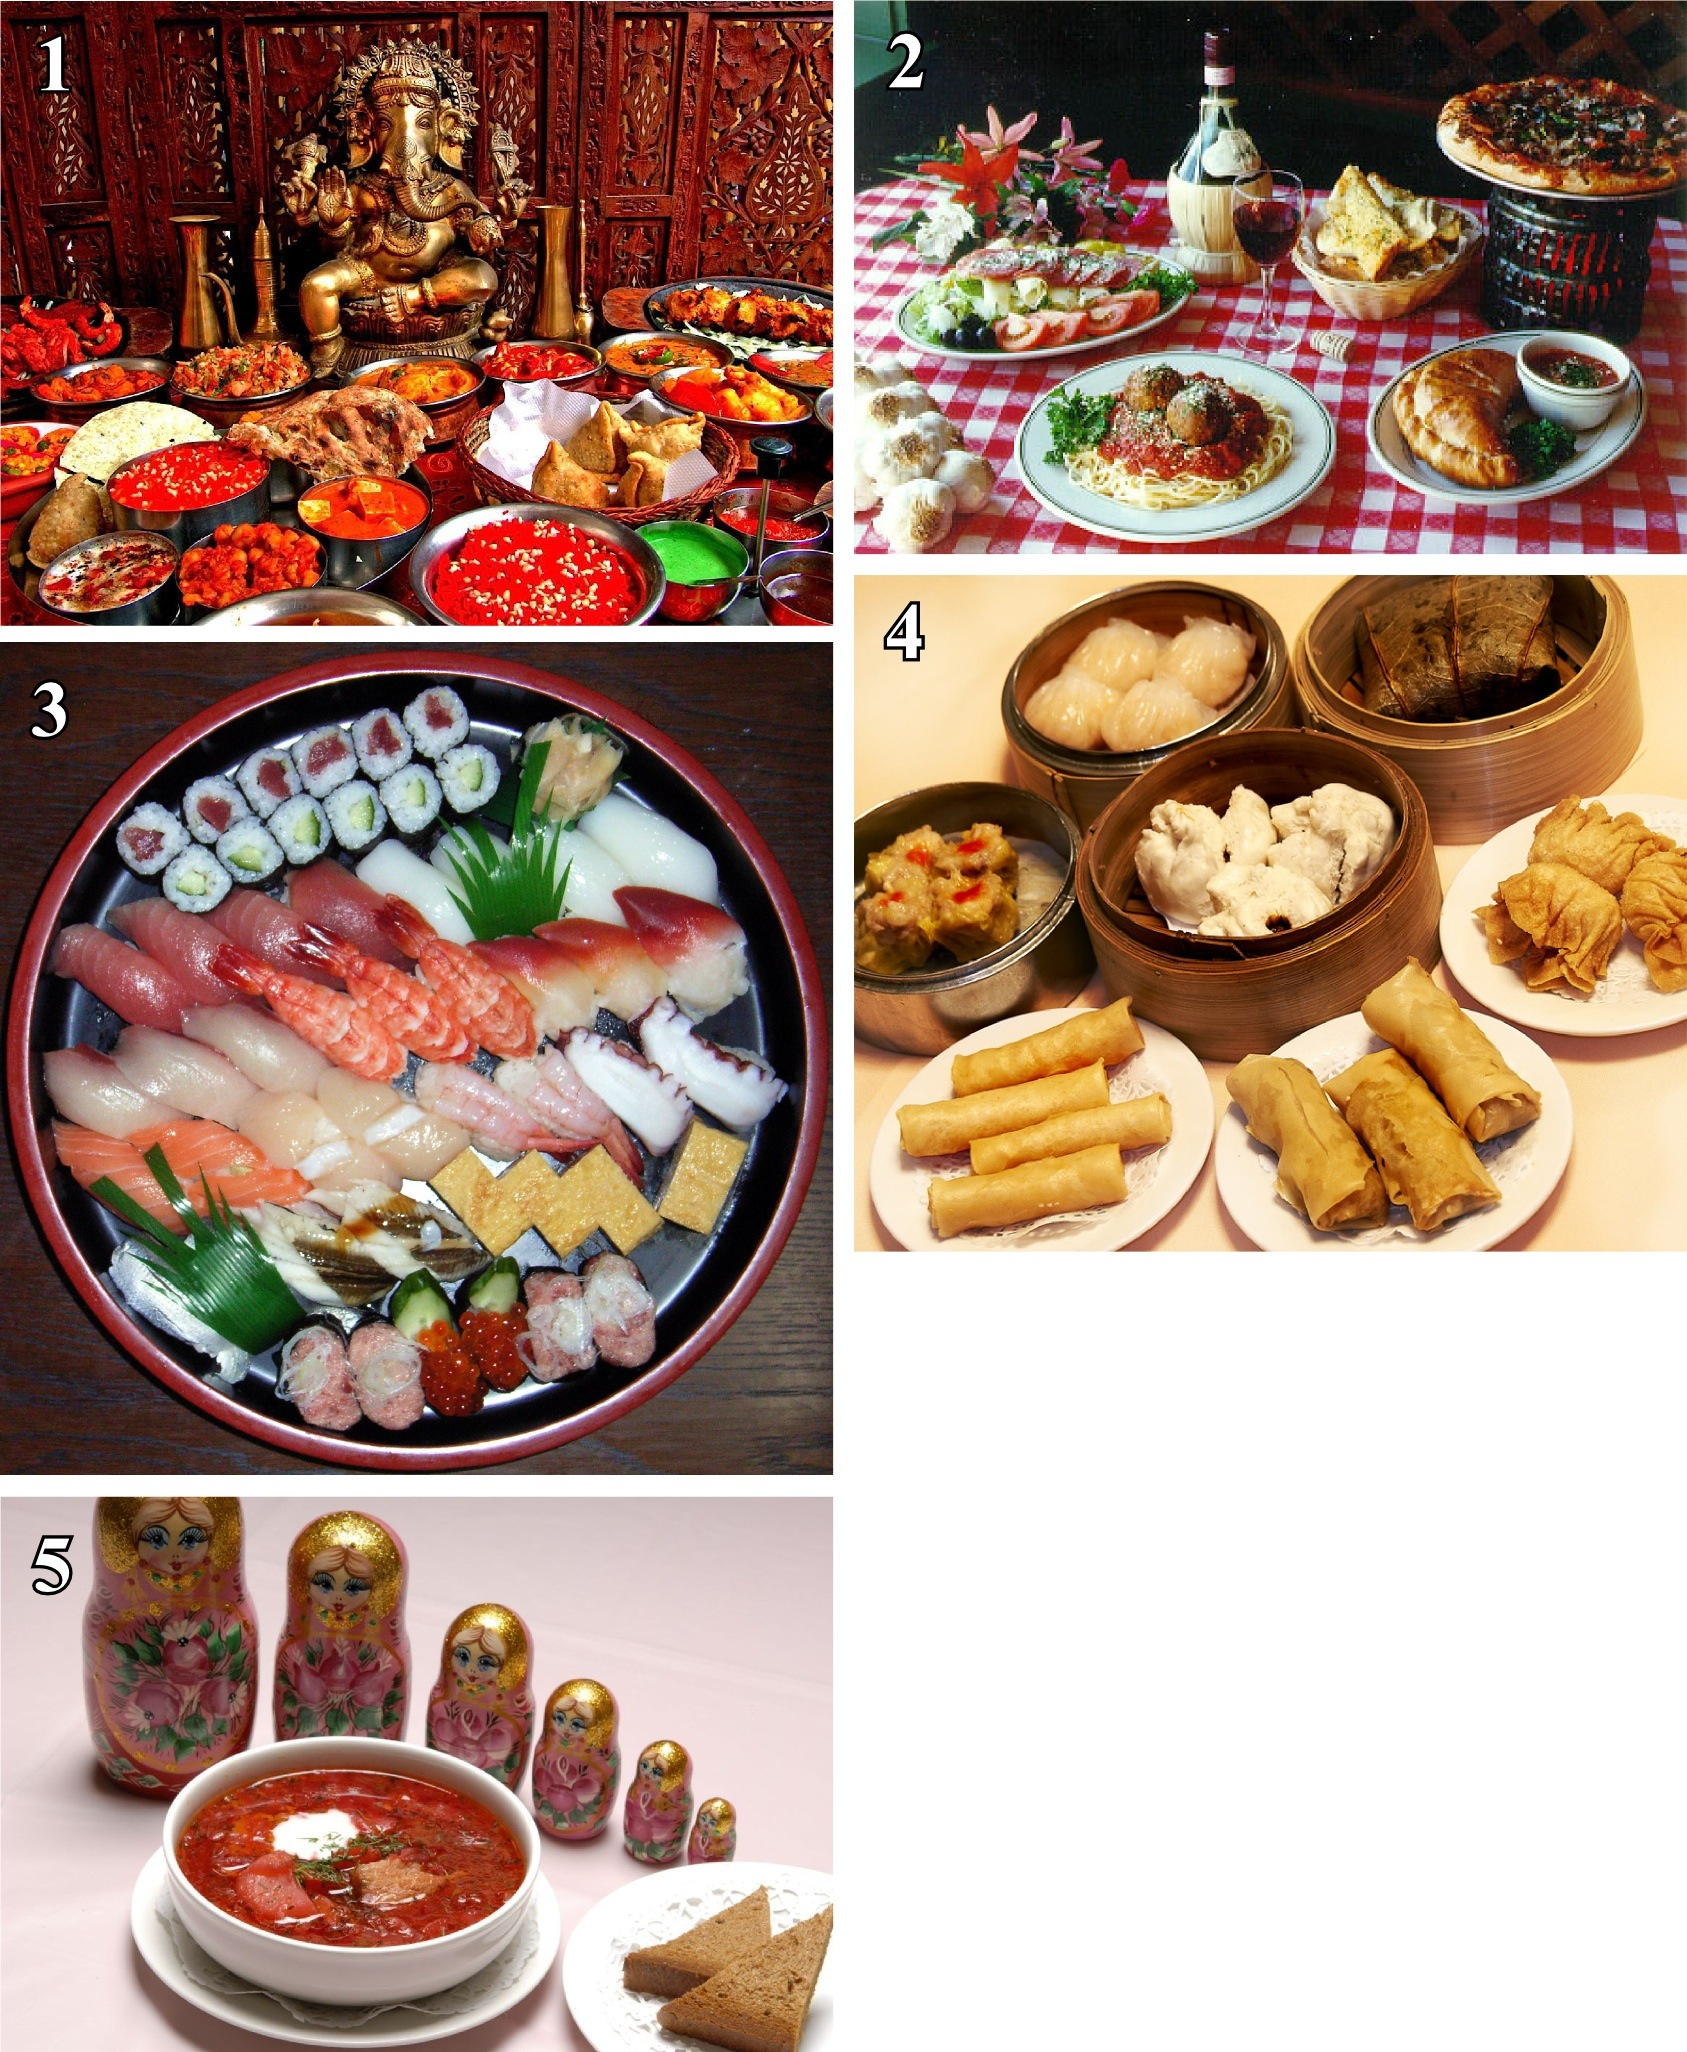
\includegraphics{figs/task2-test.pdf}
	\label{fig:task2:test}
	\caption{
		Figure S2: Images used in the test tasks for 
		\textit{exp2}.  The numbers show the order in which the 
		images were presented to workers.
	}
\end{figure}

\subsection*{S2: Access to raw data and code}
The raw data and source code needed to reproduce the analyses 
shown here and in the main text can be downloaded from 
http://networkdynamics.org/publications/public/priming2014.09.

\subsection*{S3: Additional results not shown in the main text}
		the top 5 most suppressed and most activated terms between treatment
		pairs.

\begin{table}
	\centering
	\setlength{\tabcolsep}{10pt}
	\begin{tabular}{ c c c c c }
	
		\setlength{\tabcolsep}{4pt}
		\begin{tabular}{ r | c }
		\toprule
		\multicolumn{2}{c}{\textit{task1}} \\
		\toprule
		coffee & 38 \\
		meal & 34 \\
		cheese & 34 \\
		apple & 32 \\
		dessert & 21 \\
		cup & -30 \\
		glass & -45 \\
		table & -70 \\
		candle & -74 \\
		food & -80 \\
		\bottomrule
		\end{tabular}

&

		\setlength{\tabcolsep}{4pt}
		\begin{tabular}{ r | c }
		\toprule
		\multicolumn{2}{c}{\textit{frame1}} \\
		\toprule
		bread & 18 \\
		wine & 18 \\
		cheese & 16 \\
		apple & 14 \\
		oil & 12 \\
		table & -9 \\
		meal & -10 \\
		candle & -12 \\
		dinner & -13 \\
		food & -32 \\
		\bottomrule
		\end{tabular}

&

		\setlength{\tabcolsep}{4pt}
		\begin{tabular}{ r | c }
		\toprule
		\multicolumn{2}{c}{\textit{echo}} \\
		\toprule
		apple & 24 \\
		cheese & 23 \\
		wine & 15 \\
		coffee & 14 \\
		oil & 7 \\
		knife & -24 \\
		dinner & -26 \\
		fork & -27 \\
		candle & -35 \\
		food & -55 \\
		\bottomrule
		\end{tabular}

&

		\setlength{\tabcolsep}{4pt}
		\begin{tabular}{ r | c }
		\toprule
		\multicolumn{2}{c}{\textit{task2}} \\
		\toprule
		spicy & 26 \\
		sauce & 17 \\
		indian & 15 \\
		buffet & 14 \\
		exotic & 12 \\
		festival & -11 \\
		offering & -12 \\
		statue & -15 \\
		india & -20 \\
		food & -56 \\
		\bottomrule
		\end{tabular}

&

		\setlength{\tabcolsep}{4pt}
		\begin{tabular}{ r | c }
		\toprule
		\multicolumn{2}{c}{\textit{frame2}} \\
		\toprule
		indian & 11 \\
		banquet & 8 \\
		spicy & 7 \\
		asian & 6 \\
		variety & 6 \\
		delicious & -6 \\
		meat & -7 \\
		festival & -7 \\
		spice & -7 \\
		food & -9 \\
		\bottomrule
		\end{tabular}

	\end{tabular}
	\caption{blah}
\end{table}

\subsection*{S4: Data preprocessing}
	\paragraph{Splitting, Lemmatization, removal of stop-words, and 
		addition of position tags.} 

	Before performing any analysis on the labels that workers provided, we
	performed a series of preprocessing steps.  
	\td{does this reflect the actual order in which the steps were done?}
	First, words wore lematized 
	using the
	\td{whatzit} lemmatizer.  This lemmatizer is very mild, tending only to 
	change plural words to their singular form.  Common
	words such as ``the'', ``to'', or ``with'', were found using the
	the \td{whatzit} stop-word list and removed.  Then, misspelled words were
	automatically corrected using a spelling correction algorithm described 
	below.  Finally, labels that contained
	multiple words (separated by spaces or punctuation) were split, with
	punctuation removed, and the separated words were treated as distinct 
	features in subsequent analysis.

	For the purpose of training and testing a naive Bayes classifier, we 
	performed an additional preprocessing step.  We tagged words with the
	position in which they had been entered (i.e. which of the five text 
	inputs in the task interface) as well as the test tasks in which the word 
	had been provided.
	So, if the word ``wine'' was entered into the second text-input for 
	the third test-task, after preprocessing, the feature ``3\_2\_wine'' would
	appear.  Prepending the task number onto words was simply a means to 
	retain correct attribution, which itself was essential since providing a
	word during one task is not equivalent to providing the same word during 
	another task.  
	
	\paragraph{Spelling correction.}  
	Spelling correction was performed using an algorithm that first detected
	if a word was likely to be misspelled, then generated a set of candidate 
	corrections, and chose the best candidate based on a scoring mechanism.
	
	A word was considered misspelled if it was not contained in the 
	\textit{legal set}, which was formed by the union of
	the wordnet corpus, the stop-word list, and a set of words seen while 
	crawling the world food section of the allrecipes.com website.  We
	describe the crawling of the allrecipes.com website in a section below.

	To correct misspellings, we first produced all possible modified forms 
	that could be obtained applying one or two edits.  An edit consisted of 
	adding or removing a letter, changing one letter into another, or 
	swapping the positions of two adjacent letters.  For the purpose of these 
	edits, spaces were treated as any other letter.

	The candidates produced by these edits which were in the legal set were
	then ranked based on a scoring mechanism, and the highest scoring word
	was chosen as the correction.  A candidate $w$'s score, $s_w$, was 
	calculated according to the following formula:
	\begin{equation}
		s_w = (f_w + 1) * p_1 * p_2,
	\end{equation}
	where $f_w$ is the frequency with wich the word occured (correctly 
	spelled)
	within the given task, $p_1$ was a penalty for the first edit, and
	$p_2$ was a penalty for the second edit.  If the word was made using only
	one edit, then $p_2 = 1$.  Any edit that did not involve adding a space
	(i.e. separating a word) incured a penalty of 0.5, while the addition of
	a space incurred a penalty of 0.1.  Word-separation edits were more 
	strongly penalized because it is often possible to split a series of 
	letters into many short two- or three-letter words, which otherwise leads 
	to many erroneous corrections.  We found that setting the penalty for
	word splitting at 0.1 worked well by testing on words taken from
	initial tasks.

	After all of our analyses had been performed, we checked the accuracy of 
	the spelling correction algorithm using three human coders.  The coders
	were shown a set of 
	500 words that were randomly sampled from the labels attirubuted during 
	test tasks (50 for each test task).  Before sampling, the labels from all
	experimental treatments, for the given test task, were pooled together.
	The coders did not know which treatment any given word came from.  
	In addition to the words, coders were shown the spelling correction 
	produced by the algorithm, as well as the image from the test task.
	The coders were asked to identify any misspelled words which had not 
	been corrected, as well as any corrections that appeared to be erroneous,
	by indicating their own correction.

	Based on this exercise, we found that, according to the human coders,
	17\% of the words were misspelled, but that after applying the 
	automated spelling correction, only 3.2\% of words were misspelled.

	\paragraph{Crawling the world food section of allrecipes.com.}
	The website allrecipes.com was accessed on 3-4 November 2014 using 
	automated scripts.  A total of 2642 recipe listings and 15621 recipe
	instruction pages were crawled.  Recipe listings were pages that provided 
	lists of recipes, and contained a title and short description for each.  
	The recipe instruction pages had lists of ingredients and preparation 
	instructions.  All of the words found in recipe titles, short
	descriptions, ingredients lists, and preparation instructions were
	collected, and saved as an auxiliary set to aument the \textit{legal set}
	used in spelling correction.
	


\subsection*{S5: Identification of food-related terms}
The wordnet corpus is composed of synsets, which are particular senses 
(meanings) and a set of word forms bearing that meaning. A given word form, 
such as ``ring'' has multiple senses (``to ring a bell'', ``a wedding ring''), 
and so can be part of many synsets.  Since the wordnet corpus was designed
to carry semantic information, the synset is the basic organizing element
of wordnet.

We chose the synsets \textit{food.n.01} and \textit{food.n.02} to act as roots
in defining which words should be considered food-related.  Any word form
belonging to a synset which was a hyponym of one of the two root synsets
identified above was considered to be a reference to food.  Here, as in the
main text, when we say hyponym, we mean either a direct hyponym, or a hyponym
of a hyponym, and so on.

This is a stringent notion of a word being a food reference.  It roughly
corresponds to whether or not a given thing is reasonably considered 
consumable.  So, ``orange'' is food, but ``salty'' is not.  Although ``salty''
would usually refer to something edible, it is not itself an edible thing.
On the other hand, ``salt'' would be considered a reference to food under 
this operationalization.

The subset of the wordnet corpus induced by the hyponyms of \textit{food.n.01}
and \textit{food.n.02} provide an extensive set of \td{X} words.  Manual
testing appeared to show that the coverage was very extensive, except in 
some cases references to ethnic foods were missing.  Since, especially in
\textit{exp2} we had images containing many ethnic foods, we decided to 
augment the wordnet corpus with words learned by crawling the world food
section of the allrecipes.com website.  

After collecting a set of words using an automated script 
(\td{described above}), we collected the set of words that had been used by
workers and which had been seen during crawling of the allrecipes.com website,
but which were not included in wordnet.  We graphted these extra words into
the wordnet hyponym-hypernym graph manually, which ensured that any references
to ethnic words learned from crawling would be properly classified as 
food references.

\paragraph{Validation of the detection of food references.}
To determine whether our extended version of wordnet provided a good approach
to detecting food-related words, we sampled 500 words from the set of labels
produced by workers and had three human coders manually decide if they were 
food-related or not.  The method for randomly sampling the 500 words was 
described in above in \td{section number}.

The coders were instructed to consider whether a word was a noun signifying
an edible item.  The guiding principle was, for the coder to ask herself,
``can I eat this X'', where X is the word she is coding.  The coders were
shown the used in the task from which the word came, to help resolve ambiguity
in the sense of the word that had been given.  Coders were also shown the 
spelling correction (if any) that the spell-correction algorithm had made,
to help interpret mispelled words \td{we describe the spelling correction 
algorithm in section X}.

We evaluated the food detection algorithm in two ways.  First, we measured
the inter-rater reliability between the three human coders and the algorithm
(treating the algorithm just like any other coder).  Second, adopting the 
majority code given by the human coders, we determined the accuracy of the
food-detection algorithm.  Data sumarizing this validation process are given
in table S1.

\begin{table}
\centering
\setlength{\tabcolsep}{12pt}
\begin{tabular}{ r | c }
\toprule    
\# terms coded & 500 \\
\# food references & 130 \\
\# correct machine codes & 440 \\
inter-rater reliability & 82.4\% \\
human-machine code agreement & 88\% \\
%machine recall & 80 \% \\
%machine precision & 75.4 \% \\
%machine code F1 & 0.78 \\
\bottomrule
\end{tabular}
\caption{\footnotesize{
	\td{remove the automatic numbering}. Table S1. Results for the validation 
	of the automatic detection of food references, by comparison to
	human-generated coding on randomly sampled words.  In calculating the 
	human-machine code agreement, the majority human code was used.
	Inter-rater reliability was calculated as Krippendorff's alpha.
}}
\end{table}

The results show that good inter-rater reliability was achieved during the
validation (82.4\%).  Looking at the agreement between the 
machine codes and the majority human-generated codes, we find they agree
88\% of the time.  This means that the concept used to instruct human coders
provides a good approximation to what the wordnet-based machine codes actually
represent. In other words, the machine codes correspond closely to indicating
which words correspond to nouns that refer to edible things, and which ones
don't, which provides a clear and simple interpretation for the machine
coding of food and non-food words.

\subsection*{S6: Calculation of relative specificity}
In the main text we present results for the relative specificity of labels
produced by two experimental treatments.  In performing this calculation,
we used the wordnet corpus, which has a set of hypernym-hyponym relationships
as described in the main text.  The first step in performing this calculation
was therefore to map the words occuring from (the labels of) a given 
experimental treatment onto the wordnet synsets.  In general, a given word
form can have multiple meanings, and therefore maps onto multiple wordnet 
synsets.

The result of mapping the words from two treatments onto the wordnet 
hypernym-hyponym graph two sets of counts, one set per treatment, 
indicating the number of times a word from a given synset occured among the
labels of the treatment.  Then, for every synset in one treatment, we looked
at the number of synsets in the other treatment that were more generic
(reachable by following hypernym relations) less the number of words that
were more specific (reachable by following hyponym relations).  This quantity
tallied for all words in the original synset gives a (non-normalied) measure
of the degree to which words from the first treatment are more specific
than words from the second treatment, overall.  We then normalized this 
quantity by the total number of possible comparisons between the words of
one treatment to those of the other, where two words are considered comparable
only if one word is the hypernym or hyponym of the other.  Hence, ``statue'' 
and ``bread'' are not comparable, but ``pumpernickel'' and ``bread'' are.

This calculation can be summarized by the following equation:
\begin{equation}
	S(P,Q) = \frac{
		\sum_{w\in P}\sum_{v\in Q} \left(
			\mathbf{1}_{[w>v]} - \mathbf{1}_{[v>w]} \right)
	}{
		\sum_{w\in P}\sum_{v\in Q} \left(
			\mathbf{1}_{[w>v]} + \mathbf{1}_{[v>w]} \right)
	},
\end{equation}
where $P$ and $Q$ are sets of synsets, and $\mathbf{1}_{[w>v]}$ evaluates
to 1 if synset $w$ is more specific than (i.e. is a hyponym of) synset $v$.
This measure counts the excess of cases where synsets from $P$ are more
specific then synsets from $Q$, as a fraction of all comparable synset pairs. 

In computing this quantity between two treatments, we first computed it 
using the labels attributed to a particular test task, and then
averaged the result obtained in this way for each of the five test tasks.

\subsection*{S7: Analysis of variance}
	\paragraph{Variance in the average fraction food-related labels}
	In the main text, Fig.~\ref{fig:specificity}A shows the difference in 
	the fraction of food related labels used by workers in from different 
	treatments.  The error bars show the 95\% confidence intervals around 
	the estimated difference of means.  It was computed from the
	observed sample standard deviation in the fraction of food labels given
	by individual workers.

	\paragraph{Variance in food vocabulary size.}
	\td{Not sure how to calculate this yet.}

	\paragraph{Variance in food specificity.}
	\td{Need to calculate this using bootstrapping.}


\subsection*{S8: Measuring computational hysteresis}
	\paragraph{Using cross-validation accuracy to lower-bound L1-distance.}
	In order for Eq.~\ref{l1} to be applicable, it is necessary to obtain
	an unbiased estimate of a classifier's performance.  One well-known
	pitfall in measuring this error is to underestimate it due to 
	over-fitting of the data used.  As an example, if one were to try 
	a large number of classifiers, eventually one would find one that
	classifies the data perfectly, even though it might non generalize to
	new data.

	It is customary to use part of a data set to optimize hyperparameters of
	a model, and then test the model on as-yet unseen data.  In our case,
	don't have enough samples in each treatment to do this.  Instead, for 
	this reason, we make principled decisions for all of the options used
	in our classifier, and then test it's accuracy using cross validation,
	with no optimization performed on the data.  It was cruicial for 
	the statistical validity of our approach that we test our classifier on 
	each datum only once, and report these results without any optimizations
	of the classifier.

	In performing the classification we had various options, and since we
	could not optimize these choices, we made principled decisions based on
	prior knowledge from text classification applications.  We describe the
	options we faced and the choices we made below.

	\textit{whether to correct misspelled words.}  Because we used free-text
	entry for the labels, there was bound to be many spelling mistakes.
	This would tend to reduce the accuracy of a classifier, because the 
	entries ``bread'' and ``braed'' would be regarded as completely different
	features, even though they clearly correspond to the same 
	\textit{intended word}.  While no algorithm can determine a worker's 
	intentions, it is possible to check words against a corpus, and, in the
	case of a misspelled word, look for plausible corrections based on 
	edit distance.

	\textit{Lemmatization.}  In some cases it is helpful to simplify words 
	before providing them to the classifier.  For example, the words 
	``berries'' and ``berry'' only differ in number, but would normally be
	treated as completely different features.  Lemmatization ensures that
	nouns are in their sigular form, which helps to eliminate variations in
	labels that increase sparsity without conveying discriminative 
	information.

	\textit{Removal of stop-words.}  Certain very common words such as `the',
	``to'', and ``it'' are extremely common but don't help discriminate a 
	worker's exposure.  Removing these words is a common practice because
	they otherwise introduce noise into the classifier learning process.

	\textit{Whether to split multiple words.}  Although workers were 
	instructed to put one word per text input, many put multiple words.
	Theoretically the original multi-word entry might bear additional 
	information that could be useful in discerning a worker's exposure. 
	In practice, it would be necessary for that word combination to recur,
	which is unlikely.  Therefore we chose to split multi-word entries,
	using the individual words as features.  This meant that the outputs of
	some workers generated more features than those of others.

	\textit{Preserving the location of labels.}  When workers completed image
	labeling tasks, they had to fill five text inputs, which were stacked
	vertically.  Presumably, they began with the top input and proceeded 
	downwards.  It seems likely that exposure effects might influence the
	\textit{order} in which workers apply labels, so when processing the 
	labels we prepended an integer to indicate into which text input the 
	label been input.  This meant that the classifier could distinguish
	``bread'' entered into the first text input from ``bread'' entered into
	the second.  A drawback is that this increases sparsity, preventing the
	classifier from accounting for the fact that different though they are,
	these entries should be treated similarly.  For this reason, we also
	provided features to the classifier which did not encode the particular
	input that had been used.  Thus, two workers that entered ``bread''
	into different inputs would generate both a feature in common indicating
	the use of the word ``bread'', as well as distinct features, indicating
	entry of the word ``bread'' \textit{in a particular input}.

	\textit{Preserving the connection between tasks and labels.}  In many
	cases a particular label would appear in many tasks.  For example, the
	word ``food'' appears in all test tasks.  It stands to reason that
	exposure effects play out differently for different tasks, and that
	the attribution of a particular label during one task provides different
	information from the attribution of the same label during a different 
	task.  So, as we did in the case of input location, we prepended labels
	with the identity of the task in which they were added, so that the 
	two otherwise identical labels added for different tasks were treated
	by the classifier as unique features.  Unlike in the case of input 
	position attribution, we didn't include raw labels unadorned with 
	the task number.  Our rationale for this is that the task defines the 
	context in which a label is applied, and so the elicitation of a label 
	during one task represents a distinct output from the elicitaiton of the 
	same label during a different task.  

\paragraph{Selection of the naive Bayes classifier.}
A great deal of work has been done in the application of classifiers to
text documents, which provides the bacground for our choice of classifier.
The Support Vector Machine (SVM) approach is known to perform well, better in 
general than naive Bayes.  However, three considerations drove us to use
a naive Bayes classifier in favor of SVM.

First, we used 119 examples (workers) per treatment, but the number of 
features
for each worker (i.e. the number of distinct labels, or modifications 
thereof produced in preprocessing), was generally in the thousands.  
This tends to
be problematic for many classifier algorithms, including SVM, because it
leads to very high variance models, which manifests as overfitting and poor
performance.  To deal with this, some approach to culling features is 
generally used, but this raises the issue of how to decide the culling in 
a principled manner, generally adding further hyperparameters which could
be optimized.  However, one of the strengths of the naive Bayes classifier
is that it's performance is not generally degraded from the inclusion of 
large numbers of features, even when the number of examples is comparatively
small.  We expected this feature of the naive Bayes classifier to be 
advantageous in our case.

Second, the standard implementation of the naive Bayes classifier has no 
hyperparameters to optimize.  This allows us to forgo the common practice 
of holding out a test set, and instead use cross-validation as a method to
estimate the true classification error, \textit{since we did not perform
any kind of model selection or optimization whatsoever using our data}.
This point is crucial, because if we did optimize our classifier during 
cross-validation, then the validation error would no longer provide an 
unbiased estimate of the true classification error, but would instead lead
to us over-reporting exposure effects.

Third, the naive Bayes algorithm is based on an assumption that the 
probability of observing one feature is independant from the observation
of any other, \textit{when conditioned on the class}.  This
\textit{conditional independance} assumption is generally made for
pragmatic rather than theoretical reasons, and is rarely satisfied.  However,
if it \textit{is} satisfied, then the naive Bayes classifier is optimal.
In our case, conditional independence means that, provided we know the 
exposure of a worker, knowing one label they provided to an image does
not in any way help us guess any other label for that image.  In most
text documents, the existence of topics and language structure certainly
vioalates the conditional independance of words.  But in our case, such 
effects are less likely to carry from one text input to the next, and in the
small space provided by five inputs, any overarching topics are likely to
be in relation to the image itself, upon which we are conditioning.  In other
words, we believe that, in our setup, conditional independence is better 
satisfied than in most text classification contexts.  That being the case,
one would not expect much improvement in using a more sophisticated algorithm,
such as SVM.

\paragraph{Comparison to other classifiers.} 

\begin{figure}
	\centering
	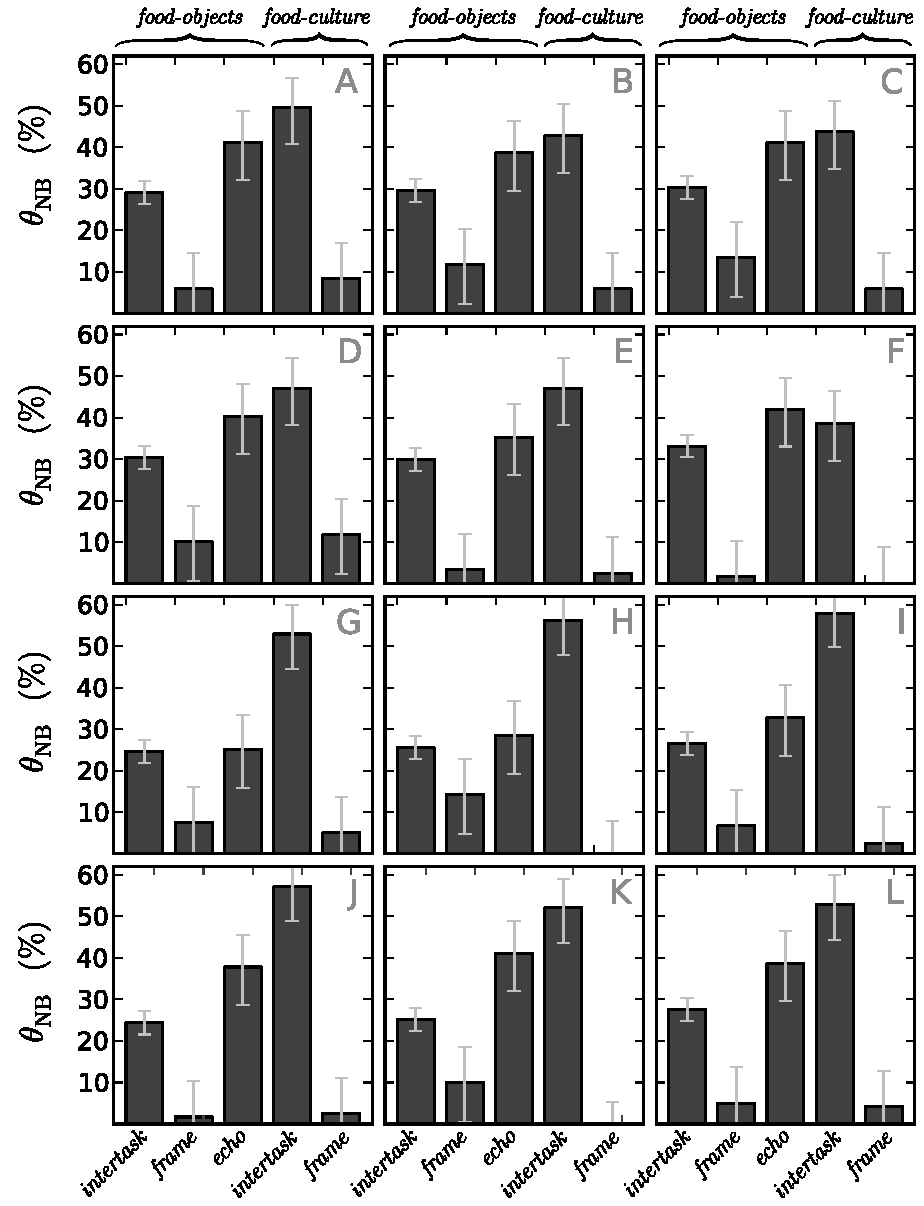
\includegraphics[scale=0.75]{figs/theta_sup.pdf}
	\label{fig:theta_sup}
	\caption{
		Figure S2: Bias induced by exposure to initial tasks and frames.
		Bias is defined to be the difference in the probability 
		distribution over workers' labels (L1-distance).  The plotted values
		give a lower bound to the L1-distance, $D_{L1}^-$, which was 
		determined from a classifier's performance in 
		distinguishing workers that had undergone different exposures.
		The bias was determined using (A-F) a naive Bayes classifier, and 
		(G-L) an SVM classifier.
		In panels A through F, each plot adds an additional
		preprocessing step to those used in the previous plot; the same is 
		done for panels G through H: A,G) No 
		preprocessing; B,H) spelling correction; C,I) stopword removal; 
		D,J) lemmatization; E,K) splitting of multiple-word labels; 
		F,L) distinguishing identical labels entered in different form inputs.
	}
\end{figure}
The inequality in Eq.~\ref{l1}
asserts that a classifiers performance in predicting class membership
bounds the L1-distance between the distributions of features for the classes.
This bound is tight for the optimal classifier, and in general, the slack
depends on how the classifier is constructed.

Therefore there may exist a classifier that is 
significantly better than the one used to generate our results.  Even before
commiting to a particular classifier algorithm, various decisions about
preprocessing need to be made.  For example, we chose to remove stopwords,
lemmatize, split multi-word labels, distinguish the input used to enter 
labels, and correct spelling.  All of these decisions affect the classifier
performance.  The particular classifier algorithm chosen also has a strong 
effect.

Since we did not have enough data to create a separate test set, we could not
optimize these decisions.  Doing so would lead to the inflation of the 
performance, which could then only be estimated using an independant test set.
Instead, we made principled decisions as described above.

Although we cannot optimize these decisions, it is appropriate to look at
what affect these decisions had, post-hoc.  We reproduce the plot shown in 
Fig.~\ref{fig:theta}A using different combinations of pre-processing options,
and using both the naive Bayes and an SVM classifier.

Unlike the naive Bayes classifier, it is necesarry to tune the cost and 
gamma hyperparameters of the SVM classifier, as well as choose a kernel.
We used simulated annealing to optimize the cost and gamma settings in the
classification of $task2:food$ vs $task2:cult$.  For this reason, we expect
the bar for $task2$ in Fig.~S8G-J is likely to be an overestimate due to
overfitting on those data.

These plots show that the result shown in Fig.~\ref{fig:theta}A is 
representative, and supports the validity of the lower bounds on the 
exposures exposure effects presented in the main text, in terms of induced 
L1-distance.


\subsection*{S9: Justifications and statistical properties of classifier-based measurement of computational hysteresis}
\begin{itemize}
	\item{Relationship to L1-Distance}
	\item{Relationship to bias}
	\item{Relationship to Jenson-Shannon divergence}
	\item{Other approaches to measuring L1-distance}
	\item{Comparison to hypothesis testing using $\chi^2$}
\end{itemize}



\end{document}

